\chapter{Estado de la técnica}

\section{Neurodegeneración: Alzheimer, Parkinson y ELA}

Este libro, plantea el objetivo de transmitir de manera sencilla y clara conceptos básicos de la neurodegeneración y de las principales enfermedades neurodegenerativas, intentado simplificar algo tan complejo como el cerebro humano. \cite{Neurodeg64:online}

\subsection{Definición y concepto}

Inicialmente, se establece la definición básica de envejecimiento como principal factor de riesgo para el proceso degenerativo. A continuación, se trata superficialmente los mecanismos importantes tanto en el envejecimiento como en la degeneración, y se expone la definición del mismo en lo relacionado con el cerebro.\\

La definición del envejecimiento se centra en la pérdida de vitalidad y el aumento progresivo de la vulnerabilidad y la fragilidad.  Este proceso biológico universal, progresivo, determinado-regulado, supresor heterogéneo e irreversible, conlleva una progresiva e irreversible pérdida de la integridad fisiológica.\\

En la sociedad actual, la esperanza de vida tiende a un incremento progresivo. En los países desarrollados está en aumento, tanto la Edad Media de la población como el porcentaje de personas dentro del rango entre 85 y 100 años. Esto pone en el punto de mira la búsqueda del retraso de la aparición de enfermedades asociadas al envejecimiento.\\

Gracias a varias investigaciones, se ha descubierto que las dietas calóricas son un importante factor de disminución de las expectativas de vida. Mediante mecanismos de reprogramación que restringen la cantidad de calorías en la alimentación, se consiguió incrementar la longevidad en numerosas especies y mejorar diversas actividades metabólicas. \\

Por otra parte, ganó importancia la identificación de genes encargados de modular la longevidad. En algunos modelos animales se identificaron elementos modificadores asociados al aumento de las expectativas de vida, como por ejemplo:
\begin{itemize}
	\item Disminución del factor de crecimiento insulina-like (IGF.1)
	\item Disminución de la proteína mTOR
	\item Aumento de la actividad de las siete sirtuinas conocidas, sobre todo de la sirtuina 1 (SIRT1) mediante la ingesta de resveratrol
\end{itemize}

Otro factor fundamental en esta línea de investigación es la epigenética. Actualmente se la define como el estudio de cambios heredables en la función genética que se producen sin ningún cambio en la secuencia del ADN. Es una ciencia que estudia la forma, como los factores ambientales y de estilo de vida que influyen en la expresión final de ciertos genes. Por esto mismo, el 
epigenoma cambia durante toda la vida en función de estas variables, siendo muy flexible y conllevando grandes implicaciones en el campo de la salud.\\

Muchas de las enfermedades debidas al envejecimiento, como algunos tipos de demencia, presentan un componente epigenético. Al envejecer, se pierden grupos metilos, las neuronas disminuyen o dejan de producir determinados neurotransmisores.\\

La posibilidad de lograr un rejuvenecimiento con los cambios epigenéticos, lleva a hablar de la reprogramación celular. Esto se el método para la modificación del epigenoma.	Mediante la combinación de cuatro genes, llamados los factores de Yamanaka pudo conseguirse la detención o reversión del envejecimiento. Esto fue descubierto por Shanya Yamanaka en el 2006, al convertir una célula adulta en una célula madre pluripotente. Para evitar que haya más probabilidad de desarrollar células tumorales, se llegó a la conclusión de no permitir la finalización del proceso de transformación.\\

Los factores ambientales modulan mecanismos epigenéticos que a su vez, modulan la capacidad funcional de las células madre.  Un decline de la funcionalidad de estas, lleva a la perdida de homeostasis. Recientemente se demostró la posibilidad de obtener células funcionalmente completas a partir de células senescentes. Esto era algo inimaginable hace no tanto en la reprogramación celular, por lo que esto muestra una evidencia adicional a la reversión del envejecimiento celular. Esto podría concluir en mejoras terapéuticas para personas con progeria.\\

Por otro lado, Se sugiere la existencia de un reloj metabólico que controla el envejecimiento. Este Se basa en 9 sellos distintivos del envejecimiento, los cuales los podemos clasificar en 3 categorías. En La primera, nos encontramos con las principales causas del daño molecular, Como la inestabilidad genómica Basada en la rotura del equilibrio entre los daños y la capacidad de reparación; Alteraciones epigenéticas que cambian la estructura del ADN; pérdida de proteostasis Y desgaste del telómero. La segunda categoría están los componentes beneficiosos a niveles bajos y dañinos a niveles altos. Entre ellos se encuentran la disfunción mitocondrial, la senescencia celular, o la detección desregulada de nutrientes. Por último, Se encuentran los elementos con los que desaparece la capacidad de autorregulación, Como el cansancio de células madre y las alteraciones en la comunicación intercelular.\\

La neurodegeneración consiste en el deterioro de células y tejidos, haciendo que estos pierdan de forma gradual la capacidad para realizar sus funciones. Por otra parte, esta la regeneración, proceso donde se restablecen células, tejidos y órganos. En cambio, las neuronas son células postmitóticas no tienen la habilidad de dividirse ni remplazarse, por lo que envejecen por la acumulación de daños con el paso del tiempo. Esto lleva a una pérdida de neuronas que afecta sobre todo al hipocampo y a los cingulados anterior y posterior, zonas especialmente afectadas en las enfermedades neurodegenerativas. También supone una pérdida de dendritas y sinapsis. 
Hay varios mecanismos encargados de inducir la neurodegeneración. Entre ellos encontramos factores diversos como pueden ser genéticos y ambientales, las dinámicas anormales de las proteínas o el daño oxidativo.   Todo esto junto con otros sistemas llevan a la muerte celular.\\

Intentando aclarar el mecanismo de degeneración de las células, algunos científicos llegaron a la conclusión de que la agregación de proteínas alteradas o deficientemente plegadas eran una de las principales causas de la muerte neuronal. Las distintas enfermedades neurodegenerativas tienen esta característica en común. Mediante distintos estudios, se consiguieron identificar ciertas alteraciones de proteínas correspondientes a diferentes enfermedades. Como, por ejemplo, el Alzheimer se asocia a la proteína B amiloide y el Parkinson a los depósitos de alfa-sinucleína.  Aún así, siguen abiertas ciertas preguntas, como el por qué de que algunas proteínas se plieguen de forma anormal y por qué algunas son más propensas a la agregación que otras.
Otro concepto muy importante y bastante reciente es la resiliencia. Esta consiste en la capacidad de los individuos a ajustarse a situaciones adversas o, en el ámbito de la física, es la capacidad de ciertos materiales para recuperarse de ciertas cargas. Los factores determinantes de la resiliencia pueden ser determinantes para las investigaciones de la neurodegeneración.

\subsection{Bases moleculares y celulares de la degeneración}

El conocimiento de las bases moleculares y celulares de la neurodegeneración son esenciales para desarrollar nuevos métodos diagnósticos así como nuevas terapias. En el libro se aborda la compleja interacción entre los diferentes procesos biológicos y fisiológicos que pueden influir en la patogénesis de diferentes enfermedades. Se ha hecho un enorme esfuerzo en estudiar los mecanismos que regulan la muerte celular, ya que esto permitirá avanzar en nuevas intervenciones terapéuticas que detengan o enlentezcan el proceso neurodegenerativo.\\

Se describen tres tipos de muerte celular: la apoptosis o “muerte celular programada”, la necrosis que se produce como consecuencia de la acción de toxinas, generando una caída de ATP y la autofagia. Este último, es un mecanismo empleado por las células eucariotas para degradar sus componentes con vistas a la renovación y recambio de estos. Se concluye que en la neurodegeneración la autofagia está descontrolada. Después de analizar este mecanismo en las principales enfermedades degenerativas, se concluye que se encuentran involucrados de una manera directa defectos en su funcionamiento.\\

Otro de los procesos objeto de estudio es la oxidación y el estrés oxidativo. Esto es debido a nuestra naturaleza como seres vivos que consumen oxígeno y que están expuestos de manera permanente a subproductos tóxicos conocidos genéricamente como  “radicales libres de oxígeno” y “radicales libres de hidrógeno”. Uno de los radicales libre de mayor interés en medicina es el óxido nítrico, se estima que tiene un papel protagonista indirecto en la neurodegeneración a través de un derivado denominado “peroxinitrito”. Los resultados de diferentes estudios demuestran que la generación de prooxidantes es un factor que influye en la velocidad de envejecimiento, el cual está relacionado directamente con el daño mitocondrial.\\

Por tanto, en el origen de las enfermedades neurodegenerativas se encuentran involucrada la elevada producción de especies reactivas de oxígeno (ROS) y especies reactivas de nitrógeno (RNS) asociadas a un mal funcionamiento de la mitocondria neuronal. El daño en el ADN, como consecuencia del estrés oxidativo, genera desarrollo de mutaciones en el mismo. En definitiva, se genera una relación multidireccional entre estrés oxidativo, mal funcionamiento mitocondrial, incremento de apoptosis y disminución de la autofagia, cuyo resultado es el desarrollo de la neurodegeneración.\\

Un último elemento a analizar es la neuroinflamación como respuesta inflamatoria del sistema nervioso central a cualquier tipo de agresión o lesión sobre este. En este punto es relevante las funciones que tiene la glía, células que desempeñan un papel esencial de soporte a las neuronas y a ala fisiología del sistema nervioso. Aunque el proceso inflamatorio es un mecanismo de defensa del organismo contra la infección, la pérdida de su regulación hace que contribuya a una condición patológica, pues mantiene un proceso de destrucción celular progresivo. Esto nos lleva a que las respuestas inflamatorias se mantienen activadas durante el estado de estrés oxidativo, lo que lleva a las neuronas a un círculo vicioso de muerte y destrucción.	

\subsection{Enfermedades neurodegenerativas}

Las enfermedades degenerativas tienen cada vez mayor protagonismo en nuestra sociedad debido al envejecimiento de la población. Se definen como aquellas patologías heredadas o adquiridas, en las que se produce una disfunción progresiva del sistema nervioso central. Existen más de 600 enfermedades neurodegenerativas, pero destacan la enfermedad de Alzheimer (EA), la enfermedad de Parkinson (EP), la enfermedad de Huntington (EH) y la esclerosis lateral amiotrófica (ELA).

\subsubsection{Enfermedad de Alzheimer}

La EA es actualmente un problema de primer orden y una prioridad para los sistemas de salud. Hay varios estudios sobre su prevalencia, el estudio Delphi prevé que en el 2040 habrá más de 80 millones de personas afectadas por la enfermedad, existiendo unanimidad en que la prevalencia se dobla cada cinco años. Siendo una de las principales causas de muerte no se puede prevenir, curar ni siquiera ralentizar su avance.
La edad es el principal factor de riesgo para su desarrollo, y presenta mayor incidencia en el género femenino en edades avanzadas, también un abaja escolarización aumenta el riesgo. Existen multitud de estudios sobre los diferentes factores de riesgo, una relación compleja difícil de interpretar debido a la alta variabilidad. La mayoría de los casos se considera que no tienen origen genético. Sin embargo, existen pruebas de factores genéticos que puedan conllevar una mayor predisposición a padecer la enfermedad, confirmándose el genotipo apolipoproteçina E (ApoE) como factor de riesgo en múltiples estudios.
En la corteza cerebral, la sustancia blanca contiene los axones (responsables de las conexiones entre neuronas). La pérdida de sinapsis podría constituir la vía final común de la patología, ya que su número disminuye con la evolución de la enfermedad.\\

Existe la necesidad de definir el estado entre normalidad y demencia y para ello han surgido en los últimos años diferentes criterios, cobrando especial relevancia en el mundo científico el término “deterioro cognitivo leve”. Los pacientes se quejan básicamente de pérdida de memoria, pero pueden manifestar otras dificultades. Las técnicas de neuroimagen son de indudable interés clínico, de forma complementaria a las manifestaciones clínicas. El objetivo es identificar a aquellos pacientes con mayor riesgo de desarrollar una demencia, e instalar un acercamiento terapéutico de manera temprana.
La demencia es un proceso progresivo. Al déficit de memoria se van añadiendo dificultades del lenguaje, la desorientación y la desorganización de las actividades cotidianas. Entre otras manifestaciones clínicas se encuentra la apraxia y la agnosia y la afasia en sus diferentes manifestaciones. Los síntomas psicológicos y conductuales afectan a los pacientes con demencia, con una prevalencia del 90\%, entre los que cabe destacar la apatía, la agresividad, así como las alucinaciones y la alteración del ciclo vigilia-sueño. Es relevante ubicar al paciente en el estadio evolutivo para programar adecuadamente su tratamiento.\\

El diagnóstico sigue siendo fundamentalmente clínico. Aunque en la ayuda al diagnóstico se empiezan a incorporar diversos biomarcadores, así como técnicas de imagen como la resonancia nuclear magnética, la tomografía por emisión de fotón único (SPECT) o la tomografía por emisión de positrones con fluordeoxiglucosa (PET-FDG). Esta última ha demostrado su utilidad para distinguir pacientes con EA de otras demencias. Otras técnicas de imagen pueden ser útiles para el diagnóstico precoz y el seguimiento de la enfermedad.\\

La intervención terapéutica debe contemplar tratamiento farmacéutico, intervención no farmacológica,  y la actuación sobre familiares/cuidadores. El tratamiento farmacológico se centra en paliar la degeneración neuronal, potenciar la actividad de las neuronas no afectadas y aliviar los síntomas de la enfermedad. El tratamiento se centra en dos grupos de fármacos: los inhibidores de acetilcolinesterasa (IACE) y los antagonistas de los receptores N-Metil-D-Aspartano tipo memantina. Una línea abierta de investigación es la búsqueda de tratamientos que sean modificadores de la historia natural de la enfermedad, destacando el dirigido contra la proteína beta amiloide o la inmunoterapia activa. En lo que respecta a las intervenciones no farmacológicas, cabe destacar: programas de orientación a la realidad, terapia de reminiscencia, terapia de validación, estimulación cognitiva y estimulación magnética. Entre las medidas aplicadas al cuidador, señalar las orientadas a los programas de información y formación, los equipos de soporte domiciliario y las unidades de apoyo sociosanitario.\\

En términos de coste económico, se considera que las demencias son la tercera causa más costosa, tras el cáncer y las enfermedades cardiovasculares. En más del 80\% de los casos, el cuidado lo realiza la familia. El diagnóstico precoz y el empleo de alternativas no farmacológicas podrían reducir el coste total de las demencias.		

\subsubsection{Enfermedad de Parkinson (EP)}

Es un trastorno neurodegenerativo crónico de curso progresivo y evolución prolongada, caracterizado por la pérdida de neuronas dopaminérgicas. Se trata de la segunda enfermedad neurodegenerativa más frecuente en mayores de 65 años, tras la enfermedad del Alzheimer y afecta entre el uno y el dos por ciento de la población. En la mayoría de los casos es de tipo esporádico y de causa desconocida.\\

Las manifestaciones iniciales suelen pasar desapercibidas. Un síntoma común suele ser el temblor en reposo y de tipo asimétrico que afecta a la mano, aunque pueden aparecer otros síntomas iniciales. Existen una serie de síntomas no motores cuya presencia puede poner sobre aviso: trastornos en el olfato, alteraciones en la fase REM de sueño y el estreñimiento. El diagnóstico precoz a través de biomarcadores es primordial, desde técnicas de neuroimagen hasta marcadores genéticos, moleculares y tisulares. Las principales manifestaciones clínicas son: Bradicinesia. Temblor, Rigidez e inestabilidad postural. A estos se les pueden unir otros síntomas motores de manera variable: Disfagia, Síndrome de piernas inquietas y alteraciones del lenguaje. Entra las manifestaciones no motoras se encuentran: depresión, ansiedad, apatía,  en algunos casos problemas de vejiga o de estreñimiento, excesiva producción de saliva o inadecuada deglución, así como problemas en la piel. Un diagnóstico temprano puede ser difícil por falta de biomarcadores con suficiente nivel de sensibilidad y especificidad. El infradiagnóstico se sitúa en un 24 \% y es frecuente un diagnóstico erróneo. Pueden ser de ayuda pruebas de neuroimagen funcional.\\

No hay cura para la EP, pero distintos medicamentos pueden proporcionar un significativo alivio en fases iniciales y debe continuarse durante casi toda la vida del paciente. La levopoda es el tratamiento sintomático más eficaz, permitiendo a los pacientes alargar el período de tiempo en el que poder llevar una vida relativamente normal. Otros fármacos, aunque menos eficaces en controlar la rigidez y la bradicinesia son la bromocriptina y la pergolida. La Selegilina se está utilizando también para la EP, pudiendo realzar y prolongar la respuesta de la levopoda. También se está experimentando con injertos naturales o el trasplante de células nerviosas, así como con el uso de células genéticamente producidas.\\

También es preciso un abordaje integral y multidisciplinar de la enfermedad, con el objetivo de mejorar o mantener la calidad de vida del paciente y sus cuidadores. Desde el ejercicio físico, la fisioterapia, las terapias ocupacionales, entre otras. Todas ellas suman para retrasar el deterioro.		

\subsubsection{Esclerosis lateral amiotrófica (ELA)}

La ELA es la enfermedad de la neurona motora más frecuente en adultos y se basa en la degeneración combinada de las motoneuronas superiores e inferiores. La consecuencia es una debilidad muscular que avanza hasta la parálisis. Su incidencia está entre 0,4-1,8/100000hab y año. Además, es más frecuente en hombres y la supervivencia media es de 3 años.\\

Los primeros síntomas suelen ser espasmos musculares y debilidad en un miembro o dificultad para hablar, afectando posteriormente a los músculos necesarios para moverse, hablar o comer. Sólo un 10 \% puede desarrollar deterioro cognitivo. Por otra parte, es difícil de diagnosticar de manera temprana y un método de ayuda es el electromiograma. Actualmente no existe ningún tratamiento eficaz, el único que ha demostrado prolongar la supervivencia es el riluzol. Todos los esfuerzos deben ir encaminados a conseguir mejor calidad de vida de pacientes y familiares. El avance de la enfermedad plantea decisiones de gran dificultad ética que deben ser compartidos con los pacientes y su familia.


\subsubsection{Enfermedad de Huntington}
Se trata de un trastorno neurodegenerativo con carácter hereditario autosómico dominante. Presenta tres manifestaciones clínicas principales: movimientos involuntarios bruscos, alteraciones de la personalidad y deterioro mental. Con una prevalencia de 5-10 casos por 100.000 habitantes, afecta igual a hombres y mujeres.\\

El diagnóstico se basa en las características clínicas y los antecedentes familiares confirmados por análisis genético del ADN. No existe tratamiento que cure o ralentice el avance, por lo que está orientado a mejorar la calidad de vida a través del tratamiento sintomático. Las vías de investigación incluyen la interferencia en RNA que operaría en el inicio del proceso. La asistencia sociosanitaria es clave en este trastorno.

\subsection{Intervención terapéutica}

Los condicionantes del estilo de vida tienen un profundo impacto en nuestro cerebro. Son tres los elementos principales a tener en consideración para prevenir los procesos neurodegenerativos: ejercicio físico, nutrición y actividad intelectual.\\

Hoy podemos establecer que la actividad física es uno de los mejores neuroprotectores existentes, demostrando mejores parámetros cognitivos asociados a la edad. Se sabe que el ejercicio físico influye en la capacidad de generar nuevas neuronas y nuevas conexiones, favoreciendo un incremento de las neurotrofinas que promueven mayores conexiones entre áreas del cerebro, además de su acción antiinflamatoria. Existe diferentes tipos de ejercicio (aeróbico, anaeróbico y de resistencia) que deben tenerse en cuenta en función de estado del paciente, en base a un análisis individualizado. Como conclusión, el ejercicio físico mejora la función cognitiva en adultos mayores de 50 años, debiendo incluir una duración mínima de 45 minutos en intensidad de moderada a vigorosa.\\

Por otro lado, hay que señalar que a actividad intelectual está directamente relacionada con el concepto de reserva cognitiva, como la capacidad del cerebro para tolerar diversas patologías. Existen varios factores asociados al desarrollo de nuestra capacidad cognitiva: volumen cerebral, educación y complejidad laboral, bilingüismo y actividad mental y estimulación cognitiva. Sin embargo, los estudios sobre estos aspectos están sujetos a limitaciones metodológicas, siendo necesario el desarrollo de estudios multidisciplinares que avancen en la evidencia científica.\\

Por último, no podemos dejar de hablar de la importancia del consumo de alimentos saludables como un gran aliado en la prevención de enfermedades neurodegenerativas. Diferentes estudios señalan que modificaciones nutricionales pueden tener un fuerte impacto en la salud. Más allá del papel que puedan desempeñar ciertos nutrientes, lo más relevante es la adopción de la dieta mediterránea como estilo de vida saludable. Los componentes de esta pueden actuar como factores de neuroprotección, como restricción calórica o como antioxidantes naturales. Hay pocos estudios que relacionen patrones dietéticos y enfermedades neurodegenerativas, centrándose más en alimentos aislados. Quedan preguntas por contestar, pero parece claro que la intervención deber realizarse incluso antes de la edad adulta para conseguir la mayor acción preventiva.\\




\section{Clinical variables and biomarkers in prediction of cognitive impairment in patients with newly diagnosed Parkinson’s disease: a cohort study}


\subsection{Introducción}

La enfermedad de Parkinson provoca un deterioro cognitivo consistente en la disminución de capacidades como memoria, atención o razonamiento. En etapas mas avanzadas, aparece la demencia que incapacita a los pacientes en su vida diaria. El desarrollo de métodos de predicción basados en el declive cognitivo leve en etapas tempranas, permitiría avanzar en la detección de la enfermedad. \\


La deficiencia en dopamina ha sido identificada como un indicador eficiente relacionado con el deterioro cognitivo. Además se han sugerido otros factores como la edad o el género. En este estudio se valora la inclusión de los niveles de líquido cefalorraquídeo (CSF-cerebrospinal fluid) e imágenes de transporte de dopamina (DAT) para predecir el declive cognitivo en un periodo de 2 años \cite{schrag2017clinical}.

\subsection{Métodos}
En este estudio se trabajó con la información de pacientes de la Parkinson’s Progression Marker Initiative (PPMI), en el cual se hace una evaluación clínica de dos grupos. Por una parte, se encuentran los pacientes a los que se les ha detectado la enfermedad de Parkinson y, por otra, un grupo de control formado por individuos sanos. Con las personas seleccionadas se llevó a cabo un seguimiento de dos años (Julio, 2010 - May, 2013). El grupo de control se seleccionó en base a su similitud con el de los pacientes, para poder realizar un análisis comparativo entre ambos colectivos. Para ello se utilizó un método de exclusión con algunos requisitos como: trastornos neurológicos clínicamente significativos o tener algún familiar de primer grado con Parkinson.\\

Los factores evaluados en este estudio fueron: 
\begin{itemize}
	\item Funciones motoras y no-motoras.
	\item Examen del líquido cefalorraquídeo (CSF).
	\item Imagen de emisión de fotón único con tomografía computarizada (SPECT) de ioflupano marcado con yodo-123 en DATSCAN.
\end{itemize}

Los cuales se analizaron a través de ciertas capacidades: memoria (HVLT-R), función visuoespacial (Benton Judgment of Line Orientation 15-item (split-half)), velocidad de proceso y atención, función ejecutiva y memoria de trabajo, y la fluencia. Se empleó cómo método de validación global de las citadas habilidades la escala MoCA (Montreal Cognitive Assesment). En función de los resultados de estas pruebas que se realizan durante un seguimiento de 2 años, los pacientes son clasificados en tres grupos:
\begin{enumerate}
	\item Cognición normal.
	
	No presenta ningún cambio en las habilidades cognitivas.
	
	\item Deterioro cognitivo medio.
	
	Aparecen ciertas puntuaciones en mínimo dos de los tests cognitivos  realizados, pero no llega a influir en las capacidades funcionales.
	
	\item Demencia.	
	
	Se detecta un deterioro funcional debido al decline cognitivo que afecta ala vida diaria del paciente.
\end{enumerate}

Además de las variables clínicas que se incluye en el estudio por estar relacionadas con el deterioro cognitivo(edad, género, años de educación, duración de la enfermedad, sentido del olfato, trastorno dela conducta del sueño por movimientos oculares rápidos(RBD), depresión, severidad de la enfermedad de Parkinson, ...), también se incluyen algunos biomarcadores ya nombrados anteriormente: 
\begin{itemize}
	\item Datos de imágenes DAT.
	\item Estado del APOE$\epsilon$4.
	\item Valoración del CSF (Líquido cefalorraquídeo).
\end{itemize}

En el proceso analítico de los datos seleccionados se identifican 5 pasos en su ejecución:

\begin{description}
	
	\item {\textbf{Paso 1}} Recopilación y evaluación de datos.
	
	Se recogieron datos en dos momentos clave, en la linea de base, donde se realizo el cuestionario MoCA y se tomaron imagen de DAT; y a los dos años de seguimiento. La diferencia entre estas dos medidas se guardo como el cambio en el puntaje MoCA. \cite{bland1995comparing}
	
	\item {\textbf{Paso 2}} Búsqueda de datos faltantes.
	
	Se utilizaron técnicas de imputación y análisis de regresión.
	
	\item{\textbf{Paso 3}} Pruebas de comparación de grupos.
	
	En función de la naturaleza de las variable se realizaron: pruebas chi-cuadrado	para variables categóricas, pruebas t para variables con distribución normal y pruebas de Mann-Whitney para las no paramétricas.
	
	
	\item {\textbf{Paso 4}} Análisis de regresión.
	
	En función del tipo de la variable de respuesta y del modelo se llevaron a cabo:
	
	\begin{enumerate}
		\item Análisis de regresión lineal. (variable continua)
	
		Para observar el cambio en el puntaje MoCA en función de variables independientes, fueron tanto univariadas como multivariadas. 
	
		\item Análisis de regresión logística. (variable categórica o binaria) \cite{bursac2008purposeful}
	
		\begin{enumerate}
			\item Univariada: Utilizada para hallar posibles factores de riesgo del deterioro cognitivo.
			\item Multivariada: Aplicando criterios de inclusión, se desarrollaron varios modelos incluyendo variables clínicas, imágenes DAT y biomarcadores CSF.
		\end{enumerate}			
	\end{enumerate}
		
		\item {\textbf{Paso 5}} Validación del modelo de predicción.
		
		Una vez evaluada la precisión del modelo y su capacidad mediante el área bajo la curva ROC (Característica de Operación del Receptor) y el índice R2 de Nagelkerke, se obtuvo el siguiente método de predicción del riesgo del paciente:\\
		
		\begin{equation}
			R = \frac{e^{PR}}{1 + e^{PR}}
		\end{equation}
		donde:
		\begin{equation}
			PR = \beta_0 + \beta_1 \cdot X_1 + \beta_2 \cdot X_2 + \beta_3 \cdot X_3 + \beta_4 \cdot X_4 + \beta_5 \cdot X_5
		\end{equation}
		
		\begin{itemize}
			\item $R$: Riesgo de deterioro cognitivo a los 2 años.
			\item $PR$: Puntuación de riesgo del paciente.
			\item $\beta_0$: Constante.
			\item $\beta_1, \beta_2, \beta_3, \beta_4, \beta_5$: Coeficientes de regresión asociados a las variables predictoras.
			\item $X_1, X_2, X_3, X_4, X_5$: Variables predictoras (por ejemplo, edad, género, puntuaciones clínicas, etc.).
		\end{itemize}
		
	\end{description}
	
	\subsection{Resultados}
	
	Del los 393 sujetos con Parkinson temprano de este estudio, 3 fueron excluidos por falta de información MoCA en la línea de base, 318 tenían resultados disponible cuando se descargó la información a los 2 años y a 314 se les evaluó el deterioro cognitivo. Además, cierta información de algunas variables se fue perdiendo a lo largo de la investigación, pero no llego a alterar los resultados finales. De los evaluados, al final del estudio a 49 de ellos se les diagnosticó deterioro cognitivo medio, 3 pacientes desarrollaron demencia y los otros 262 se mantuvieron como cognitivamente sanos. En el grupo de control formado por 178 sujetos, solamente 2 evolucionaron a deterioro cognitivo medio.\\
	
	En los análisis multivariados, el cambio en la puntuación Moca desde el principio del seguimiento a los dos años en el grupo que padece la enfermedad se debe a: edad, puntuación UPSIT (Test de Identificación del Olor de la Universidad de Pensilvania), 
	estado APOE, y relación de A$\beta$42 a t-tau del CSF. Mientras que en el grupo saludable fue relacionado con: edad, género y CSF A$\beta$42.\\
	
	Los 52 participantes que fueron clasificados con deterioro cognitivo tenían las siguientes características al inicio en comparación con aquellos sin decline cognitivo:
	\begin{itemize}
		\item Mayor edad.
		\item Mayor puntuación RBDSQ (Cuestionario de Detección de Trastorno del Comportamiento del Sueño REM).
		\item Menor puntuación UPSIT.
		\item Menor CSF A$\beta$ y relación A$\beta$42 a t-tau.
		\item Menor captación media de caudado y
		asimetría de caudado y putaminal
	\end{itemize}	
	
	Tras realizar un análisis de regresión logística, combinando distintas variables en cada modelo y comparándolos con los resultados obtenidos para el caso de incluir solamente la edad, se llegó a un modelo final. En este se combinaron las variables relacionadas fuertemente con el deterioro cognitivo en análisis univariados (edad, puntuación UPSIT, puntuación RBDSQ, CSF A$\beta$42 y captación media del caudado). Este obtuvo un AUC (Área Bajo la Curva) de 0.80 y p = 0.0003. También se detecto una diferencia significante en el valor AUC entre el modelo final y los modelos usando la edad junto con variables clínicas o parámetros CSF. Mostrando el modelo final en una tabla en función de la edad y las distintas variables se llego a la conclusión de que se puede eliminar la captación del caudado sin influir en las puntuaciones de otras variables, ya que su relación con el deterioro cognitivo no es clara. Por otra parte, con la validación cruzada se confirmo que el modelo final es consistente con las diferentes muestras (p=0.88).\\
	
	\subsection{Conclusiones del estudio}
	
	En este estudio, siguiendo los objetivos marcados, se encontraron factores clínicos y señales biológicas que pueden predecir el decline cognitivo en los primeros dos años tras diagnosticarse el Parkinson. Este deterioro, relacionado fuertemente con la aparición de demencia en personas que padecen esta enfermedad, se asoció con varios aspectos clínicos independientemente del resultado obtenido a los dos años. Los resultados de la investigación muestran que la edad, los síntomas clínicos y ciertos biomarcadores pueden predecir la disminución cognitiva en etapas tempranas de la enfermedad. Gracias a las combinaciones de variables obtenidas en este estudio, podrían llevarse estos conocimientos a prácticas y ensayos clínicos para identificar personas en riesgo de deterioro cognitivo, aunque también serían necesarios estudios adicionales para confirmar estos resultados.\\
	
	
	
	
	\section{Statistical analysis of longitudinal neuroimage data with Linear Mixed Effects models}
	
	
	\subsection{Introducción}
	En resumen, los estudios de neuroimagen longitudinal (LNI) están en auge debido a su capacidad para proporcionar un mayor poder estadístico y comprender la dinámica temporal de procesos biológicos. Sin embargo, a menudo carecen de herramientas estadísticas maduras y sofisticadas debido a la complejidad técnica y a la falta de software de fácil uso.\\
	
	Los Modelos Lineales de Efectos Mixtos (LME) se destacan como un marco estadístico flexible y poderoso para analizar datos longitudinales. En este artículo, se comparan los fundamentos teóricos de los LME con otros métodos comunes utilizados en LNI, como el Análisis de Varianza (ANOVA), el análisis transversal de mediciones resumidas y estrategias de dos etapas. Se demuestra que los métodos convencionales presentan limitaciones, como la incapacidad para manejar tiempos imperfectos o datos desequilibrados.\\
	
	Además, se describe y analiza el enfoque del modelo lineal (LME) para estudios longitudinales, junto con las herramientas computacionales que lo implementan. Se utiliza una base de datos de resonancia magnética estructural longitudinal de la Iniciativa de Neuroimagen de la Enfermedad de Alzheimer (ADNI) para ejemplificar la aplicación de estos métodos en diferentes funciones de análisis.\cite{bernal2013statistical}
	
	\subsection{Métodos y materiales}
	\subsubsection{Características de datos longitudinales}
	
	Los datos longitudinales son un método para estudiar los resultados midiendo repetidamente variables en una cohorte de individuos en múltiples momentos. Así, se analizan los cambios a lo largo del tiempo y su asociación con factores clínicos, experimentales o biológicos. Permite la evaluación directa de los cambios dentro del sujeto en diferentes momentos, lo que permite estimaciones y predicciones más precisas sobre la trayectoria de medición de un individuo.\\ Los datos longitudinales exhiben varias características distintivas:
	\begin{itemize}
		\item Están ordenados en el tiempo. Reflejan la trayectoria temporal de un proceso continuo no estacionario subyacente.
		\item Están típicamente correlacionados positivamente para mediciones en serie para un solo sujeto.
		\item No son una variación constante entre sujetos durante la duración del estudio
		\item Es común la falta de datos y los tiempos de medición no uniformes.
	\end{itemize}
	
	\subsubsection{Modelado Lineal de Efectos Mixtos para datos longitudinales}
	
	El modelado lineal de efectos mixtos (LME) es un método estadístico utilizado para datos longitudinales que modela la trayectoria de medición media a lo largo del tiempo y la estructura de correlación entre mediciones en serie. LME utiliza el paradigma de regresión lineal \cite{montgomery2021introduction} para describir la medición promedio y su trayectoria temporal, lo que permite datos desequilibrados.\\
	
	Hay tres fuentes con potencial de variabilidad que influyen en la estructura de correlación en los datos longitudinales: la variación entre sujetos, el cambio biológico inherente dentro del sujeto y el error de medición. Los modelos LME también proporcionan modelos de covarianza flexibles y parsimoniosos, ya que introduce efectos aleatorios para estructurar la covarianza.\\
	
	El modelo LME se basa en la siguiente ecuación:
	\begin{equation}
		Y_{i} = X_{i}\beta + Z_{i}b_{i} + e_{i}
	\end{equation}
	
	Donde $Y_{i}$ es el vector $n_{i}\times1$ de mediciones en serie para el sujeto i, $n_{i}$ es el número de mediciones en serie específicas del sujeto, $X_{i}$ es la matriz $n_{i}\times p$ de diseño de sujetos para efectos fijos, $\beta$ es un vector $p\times 1$ de coeficientes de regresión de efectos fijos desconocidos, $Z_{i}$ es la matriz de diseño $n_{i}\times q$, con $q\leq p$ para efectos aleatorios, y $b_{i}$ es un vector $q\times 1$ de efectos aleatorios y $e_{i}$ es un vector $n_{i}\times 1$ de errores de medición.\\
	
	El modelo distingue entre los medios convencionales y marginales, siendo la media condicional o específica de $Y_{i}$:\\
	\begin{equation}
		E(Y_{i}|b_{i}) = X_{i}\beta + Z_{i}b_{i}
	\end{equation}y la media marginal o promediada poblacional de $Y_{i}$:\\
	\begin{equation}
		E(Y_{i}) = X_{i} \beta
	\end{equation}
	siendo $\beta$ el parámetro de regresión de la población e I coeficientes de regresión específicos del sujeto.\\
	
	
	El modelo LME permite el análisis explícito de fuentes de variación entre sujetos (D) y dentro de los sujetos ($\sigma 2$), con la covarianza marginal expresada como una función de efectos aleatorios que varían en el tiempo.\\
	
	El coeficiente $\beta$ y los parámetro $\sigma $ y D son desconocidos. Por ello, para su estimación se utilizan los supuestos distributivos del siguiente vector de medidas. 
	\begin{equation}
		Y_{i}\sim N(X_{i},\beta,Z_{i}DZ_{i}^{T} + \sigma ^{2} I_{n_{i}})
	\end{equation}
	La estimación de máxima verosimilitud de $\beta$ se hace de la siguiente forma:
	
	\begin{equation}
		\hat{\beta}=(\sum_{i=1}^{m}X_{i}^{T} \hat{\epsilon}_{i}^{-1}X_{i})^{-1} \sum_{i=1}^{m} X_{i}^{T} \hat{\epsilon}_{i}^{-1}y_{i}
	\end{equation}
	
	Mientras que $\sigma $ y D se estiman mediante el procedimiento ReML \cite{verbeke1997linear}, el cual no tiene una solución cerrada para su optimización. Entonces, se implementan tres métodos muy utilizados: 
	\begin{itemize}
		\item Algoritmo de maximización de expectativas (EM).
		\item Esquema de puntuación de Fisher.
		\item Dos métodos basados en Newton-Raphson.
		
	\end{itemize}
	
	Para determinar la estructura de covarianza de un modelo es necesario seleccionar efectos aleatorios. Una buena estrategia es el uso de la prueba de razón de verosimilitud para comparar la probabilidad de modelos anidados, siguiendo el siguiente proceso: se comienza con un modelo básico, se estiman los parámetros y coeficientes, se agregan efectos aleatorios y se evalúa la importancia de un aumento de probabilidad utilizando una estadística de mezcla de chi-cuadrado.\\
	
	Por otra parte, se realizan pruebas de hipótesis en las que se utiliza $\hat{\beta}$ y su matriz de covarianza asintótica estimada:
	\begin{equation}
		C \hat{o} v_{asymptotic}(\hat{\beta})=(\sum_{i=1}^{m}X_{i}^{T} \hat{\epsilon}_{i}^{-1}X_{i})^{-1}
	\end{equation}
	
	Las dos hipótesis que se contrastan son:
	\begin{equation}
		H0: L \beta = 0
	\end{equation}
	\begin{equation}
		HA: L \beta \neq 0
	\end{equation}
	
	Además,sabiendo que la distribución F se cumple bajo la hipótesis nula, se obtienen los grados de libertad implementando una aproximación basada en Satterhwaite para una estadística F escalada. Quedando la distribución de la siguiente forma:
	\begin{equation}
		F=\frac{\mathit{k}(L\hat{\beta})^{T}(LC\hat{o}v_{KR}(\hat{\beta})L^{T})^{-1}L\hat{\beta}}{rank(L)}
	\end{equation}
	
	
	
	\subsubsection{Estimación del tamaño de muestra y el análisis del poder estadístico}
	
	En los diseños longitudinales, es complicada la estimación del tamaño de muestra y el análisis del poder estadístico. \\
	
	Se proporcionan dos métodos aproximados para realizar cálculos de potencia: uno para planificar antes de la recopilación de datos y el otro para estimar el poder de un estudio realizado después de la recopilación de datos. En el primero, se basa en una extensión del tamaño de muestra y fórmulas de potencia para un estudio transversal con una medición univariada. Mientras que el segundo da una aproximación más precisa de la potencia de un experimento realizado, basada en una aproximación F no central a la distribución del estadístico F bajo la hipótesis alternativa. 
	
	
	\subsubsection{Métodos alternativos para analizar LNI}
	
	El análisis de datos de neuroimagen longitudinal (LNI) ha sido un tema de interés en los últimos años. Dos métodos comunes para el análisis de este tipo de datos incluyen ANOVA de medidas repetidas y valores resumidos.\\ 
	
	El primer método, que equivale a un modelo lineal con como máximo un único efecto aleatorio, es más adecuado para datos longitudinales equilibrados con un pequeño número de mediciones en serie. Sin embargo, este método no es adecuado para datos longitudinales, ya que se espera que la correlación entre mediciones repetidas disminuya con separaciones crecientes en el tiempo.\\
	
	El segundo método, que reduce la secuencia de medidas repetidas para cada individuo a valores resumidos, no es adecuado para datos no balanceados, ya que las medidas resumidas no se extraerán de la misma distribución y pueden tener una varianza diferente. Además, ignorar la correlación entre medidas repetidas y omitir sujetos con un solo punto temporal puede conducir a una pérdida significativa de poder estadístico.
	
	
	\subsubsection{Datos longitudinales del ADNI}
	
	El estudio utilizó datos de resonancia magnética cerebral longitudinal de la Iniciativa de Neuroimagen de la Enfermedad de Alzheimer (ADNI) y aplicó FreeSurfer, un proceso automático que calcula mediciones de espesor en diversas representaciones cerebrales. Esto incluye superficies corticales, segmentación de sustancia blanca, extracción del cráneo, corrección del campo de polarización, registro cortical y etiquetado de regiones cerebrales.\\
	
	El estudio se enfocó en dos biomarcadores clave para la enfermedad de Alzheimer (EA): grosor medio en la corteza entorrinal (ECT) y volumen total del hipocampo (HV). Estos marcadores están fuertemente asociados con la EA temprana. Se realizó un análisis adicional para evaluar el impacto del tipo de bobina en la medición del volumen del hipocampo, encontrando que dos tipos de bobinas afectaban significativamente las mediciones.\\
	
	En los análisis, se consideraron variables independientes como: tiempo desde el inicio, pertenencia al grupo clínico, edad inicial, sexo, genotipo APOE, educación, entre otros. Se evaluaron efectos aleatorios y se limitó el análisis a la asociación entre la interacción grupo-tiempo para HV y ECT en el ADNI longitudinal.
	
	
	\subsection{Resultados}
	En primer lugar, en este estudio se comparan las tasas de atrofia de cuatro grupos clínicos: personas sanas (HC), deterioro cognitivo leve estable (sMCI), deterioro cognitivo leve con progresión (cMCI) y pacientes con enfermedad de Alzheimer (AD), enfocándose en la atrofia cerebral.\\
	
	Tras probar diversas hipótesis, se obtuvieron diferentes resultados que afirmaron diferencias significativas en la atrofia cerebral entre estos grupos. Destacó el mayor poder de detección utilizando el grosor medio de la corteza entorrinal (ECT). Además, se proporcionaron aproximaciones del tamaño de muestra para futuros estudios que comparan las tasas de atrofia entre sMCI vs. cMCI y AD vs. HC, basadas en el tamaño del efecto y las tasas de deserción calculadas a partir de la muestra de ADNI.\\
	
	En segundo lugar, se compararon las tasas de atrofia entre sujetos sanos y sujetos con conversión de HC (cHC), que progresaron a deterioro cognitivo leve o EA con el tiempo. Se compararon las tasas de pérdida de volumen cerebral (HV) y grosor cortical (ECT) entre ambos grupos y se observó que los convertidores tenían cambios en la corteza entorrinal (ECT) que seguían un patrón no lineal. Se realizaron pruebas para comparar estas trayectorias y sus cambios a lo largo del tiempo. Los resultados indicaron diferencias significativas en las trayectorias y pendientes entre los grupos de estudio.\\
	
	Además, se evaluó cuánto poder tenían estos resultados para detectar cambios en la atrofia. En este análisis, el volumen cerebral (HV) resultó ligeramente más efectivo que el grosor cortical (ECT).\\
	
	Por otra parte, se realiza un experimento adicional que compara la metodo-logía LME con otros métodos alternativos, como el ANOVA de medidas repetidas (rm-ANOVA) y el análisis transversal de la pendiente (x-slope). Se estudió su precisión y fiabilidad en detectar diferencias entre personas sanas y pacientes con Alzheimer, concluyendo que, para grupos no muy grandes, el LME y x-slope son más efectivos. Además, el LME es más sensible a los cambios de los indicadores de la enfermedad y es más consistente entre muestras diferentes.\\
	
	Finalmente, se explora el efecto de incluir sujetos con un solo punto temporal en el análisis de datos longitudinales. Se demuestra que incluir estos sujetos puede mejorar la precisión del modelo y, por ende, mejorar la inferencia realizada en el estudio.
	
	
	\subsection{Conclusión}
	En resumen, este estudio resalta la utilidad de los modelos de efectos mixtos lineales (LME) para analizar datos de neuroimagen a lo largo del tiempo. Los LME son eficaces al lidiar con datos desequilibrados y con sujetos que solo tienen una medición, ofreciendo una forma precisa de entender cómo cambian ciertas medidas cerebrales en diferentes condiciones de salud.\\
	
	En tres experimentos, aplicaron LME a datos del cerebro para comparar tasas de atrofia en distintos grupos (personas sanas, con deterioro cognitivo, y pacientes con Alzheimer). Mostraron que los LME proporcionan sensibilidad y especificidad superiores en la detección de cambios cerebrales que otros métodos comunes. Además, demostraron que incluir a personas con solo una medición mejora la precisión de los resultados.\\
	
	En conclusión, los LME son esenciales para entender cómo evolucionan los cambios en el cerebro con el tiempo. Este estudio promueve su uso y ofrece herramientas que amplían su aplicabilidad en análisis de imágenes cerebrales a lo largo del tiempo.\\
	
	
	
	
	
	\section{Estimating long-term multivariate progression from short-term data}
	
	
	\subsection{Introducción}
	En este texto, centrado en un planteamiento de la enfermedad del Alzheimer (EA), se observa lo complejo que es el estudio del desarrollo de las enfermedades crónicas. Una de las dificultades principales es establecer un punto de inicio claro para el modelo de la progresión de la enfermedad. Esto se debe a la observación de grupos de personas en diferentes etapas de la enfermedad,  a través de "instantáneas" longitudinales a corto plazo. Además, es fundamental la utilización de biomarcadores y datos cognitivos para entender la progresión de la EA incluso antes de que aparezcan síntomas claros.\\
	
	Por otra parte, se presenta el modelo SEMOR (Self-modeling regresión) \cite{kneip1988convergence}, el cual estima a largo plazo las trayectorias del Alzheimer y otros resultados aun teniendo un conjunto limitado de datos a lo largo del tiempo. Es de gran importancia modelar curvas de progresión a largo plazo en función de múltiples medidas,ya que permite ver los cambios de los pacientes según su desempeño en las distintas evaluaciones. A parte, se habla del estudio "Personnes Agées Quid" (PAQUID) que proporciona trayectorias a largo plazo del Examen del Estado Mental Mínimo (MMSE). Esta información servirá como complemento de los datos de la ADNI para comprender mejor la progresión de la EA.
	
	\subsection{Modelo}
	El modelo propone que varios resultados $Y_{ij}$ ocurren durante un tiempo \textit{t} para individuos \textit{i=1,...,n} y marcadores \textit{j=1,...,m} según la ecuación:
	\begin{equation}
		Y_{ij}(t)=g_{j}(t+\gamma_{i})+\alpha_{0ij}+\alpha_{1ij}t+\epsilon_{ij}(t)
	\end{equation}
	
	Cada $g_{j}$ es una función monótona continuamente diferenciable con media cero y varianza $\sigma_{\gamma}^{2}$. Las tuplas $(\alpha_{0ij},\alpha_{1ij})$ siguen una distribución gaussiana con media cero y matriz de covarianza $\sum_{j}$. Los errores residuales $\epsilon_{ij}(t)$ son gaussianos e independientes con media cero y una variación específica para cada marcador.
	
	El "tiempo de observación a corto plazo" se representa mediante la covariable observada \textit{t}, mientras que el "tiempo de progresión a largo plazo" se representa por \textit{t+$g_{i}$}, donde $g_{i}$ es el desplazamiento temporal específico del sujeto. El objetivo del algoritmo es estimar tanto los parámetros temporales como las curvas a largo plazo, asumiendo que estas son monótonas y utilizando la información entre los marcadores para estimar desplazamientos temporales específicos. Este modelo es una versión simplificada del modelo SIM clásico para cada marcador, excluyendo los parámetros de reescalado pero incluyendo una pendiente adicional aleatoria.\cite{donohue2014estimating}
	
	\subsection{Algoritmo}
	Para abordar la complejidad del problema multidimensional, se desglosará en etapas con el algoritmo. Para ello se estiman los parámetros desconocidos $(g_{j}, \gamma_{i}$ y $\alpha)$ de forma secuencial, utilizando las estimaciones actuales de los otros parámetros en cada iteración hasta alcanzar la convergencia del error cuadrático (RSS). Para lograrlo, se utilizan tres tipos de residuos parciales, cada uno proporcionando una estimación imparcial de un parámetro desconocido, siempre que el modelo inicial sea correcto.\\
	
	Tras inicializar $\gamma_{i}$ a cero, comienza el proceso que se dividirá en dos etapas principales:
	\begin{description}
		\item {\textbf{Etapa 1}} Estimación de funciones monótonas y parámetros específicos para cada marcador \textit{j}
		
		Se inicia estimando las funciones monótonas $g_{j}$	y los parámetros específicos para cada marcador. Para cada \textit{j}, se utilizan subrutinas paralelas para ajustar $g_{j}$
		y los parámetros $\alpha_{0ij}$ y $\alpha_{1ij}$ específicos, utilizando un suavizado monótono \cite{10.1111/1467-9868.00130} y un modelo lineal mixto \cite{bates2010lme4}, respectivamente.
		\item {\textbf{Etapa 2}} Estimación de desplazamientos temporales $\gamma_{i}$
		
		Se invierten las variables y se estima el desplazamiento temporal $\gamma_{i}$ promediando los residuos de todos los marcadores y tiempos para cada individuo. Este paso es fundamental para lograr la convergencia del error cuadrático total.
	\end{description}
	
	El algoritmo se repite iterativamente hasta que se alcanza la convergencia deseada, logrando estimaciones precisas y refinadas de los parámetros y curvas de interés para abordar el problema complejo en estudio.
	
	\subsection{Simulaciones}
	Mediante el algoritmo diseñado en el apartado anterior, se simularon los datos del modelo y se estimaron curvas utilizando un suavizante monótono de B-spline con cinco nudos equiespaciados y splines polinómicos de quinto grado. En las imágenes siguientes, se ve como las curvas ajustadas resultantes demostraron una alta precisión al replicar las curvas logísticas, lineales y cuadráticas verdaderas .\\
	
	Además, se compararon los desplazamientos temporales reales con los estimados a partir de la simulación, aunque esta comparación no se muestra visualmente. A pesar de que no hubo una concordancia perfecta, la línea de regresión en el gráfico de dispersión estuvo cercana a la línea de identidad, como se anticipaba. El error cuadrático residual (RSS) para cada marcador convergió en 10 iteraciones, alcanzando una tolerancia del 0.1\% del RSS.
	
	\subsection{Resultados ADNI y PAQUID}
	
	El texto explora los resultados basados en datos recopilados durante el Alzheimer's Disease Neuroimaging Initiative (ADNI) y el estudio Personnes Agées Quid (PAQUID). El objetivo principal es comprender la progresión de la enfermedad de Alzheimer (AD) a través de un análisis detallado de diversos marcadores clave. Se busca derivar curvas de progresión basadas en datos reales, alejándose de las hipótesis teóricas.\\
	
	El proceso comienza con la transformación de los datos a una escala percentil. Esta transformación facilita la comparación significativa entre grupos heterogéneos, permitiendo un análisis más profundo de la progresión de la enfermedad. Se exploran trayectorias de progresión en diferentes grupos, incluidos aquellos con acumulación de amiloide y portadores de ciertos alelos genéticos. En la \ref{fig:figura1} se visualiza la progresión a lo largo del tiempo de distintos marcadores como la acumulación de amiloide en los distintos grupos.\\
	
	\begin{figure}[h!]
		\centering
		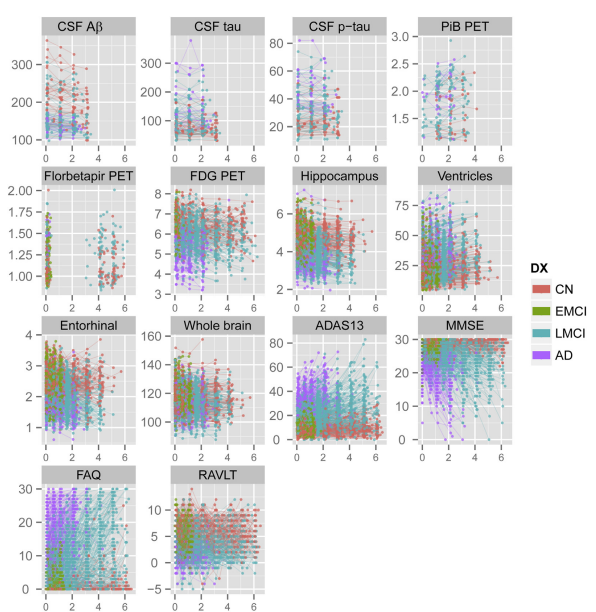
\includegraphics{fig.1}
		\caption{Iniciativa de Neuroimagen para la Enfermedad de Alzheimer (ADNI): biomarcadores, evaluaciones, categorías diagnósticas, datos longitudinales.}
		\label{fig:figura1}
	\end{figure}
	
	Se destaca la asociación entre la acumulación de placas de amiloide en el cerebro y la disminución del líquido cefalorraquídeo (CSF), junto con un aumento en la captación de PiB y florbetapir en la tomografía por emisión de positrones (PET). Se utiliza un enfoque de suavizado basado en B-spline para estimar las curvas de progresión a largo plazo, brindando una visualización clara de la evolución de la enfermedad en diferentes cohortes.\\
	
	El estudio también investiga subgrupos de sujetos, incluyendo aquellos con evidencia de acumulación de amiloide y portadores del alelo $\epsilon$4 de la apolipoproteína E (APOE). En \ref{fig:figura2} se presentan las trayectorias estimadas de dos grupos: aquellos sin evidencia de carga amiloide y aquellos sin el alelo $\epsilon$4 de APOE.\\
	
	\begin{figure}[h!]
		\centering
		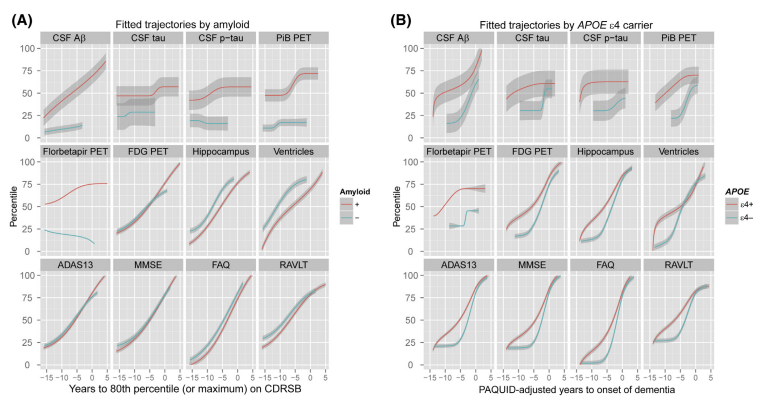
\includegraphics{fig.2}
		\caption{Comparación de portadores y no portadores del alelo APOE $\epsilon$4 en trayectorias de biomarcadores cerebrales.}
		\label{fig:figura2}	
	\end{figure}
	
	
	Se observa que los portadores de este alelo tienen una progresión más rápida de la enfermedad en comparación con los no portadores. Se emplea una transformación del tiempo para comparar las trayectorias de progresión con el estudio PAQUID, proporcionando información valiosa sobre la relación entre la carga de amiloide, la genética y la progresión clínica. 
	
	
	\subsection{Discusión}
	El texto examina la forma en que se analiza la evolución de la enfermedad de Alzheimer, utilizando datos de dos estudios: el Alzheimer's Disease Neuroimaging Initiative (ADNI) y el estudio Personnes Agées Quid (PAQUID). Se compara este enfoque con un estudio previo que se centró en cómo se hereda la enfermedad de Alzheimer, utilizando la edad en la que los padres desarrollaron síntomas para estimar la progresión de la enfermedad. Sin embargo, en este estudio, se aborda una limitación importante de ADNI al estimar tanto la edad en que se desarrollan los síntomas como las formas de evolución de la enfermedad al mismo tiempo.
	
	Además, se resaltan las diferencias en las curvas de evolución de diversos marcadores de la enfermedad, como los niveles de proteína beta-amiloide en el líquido cefalorraquídeo (CSF), la proteína tau, los resultados de tomografía por emisión de positrones (PET) con el compuesto Pittsburgh Compound B (PiB), el metabolismo de la glucosa y el tamaño del hipocampo. Se sugiere que estos marcadores siguen trayectorias distintas y que algunos tienen una evolución más constante, mientras que otros muestran un patrón de crecimiento y descenso.
	
	Por otra parte, se menciona la influencia de factores como la genética, la dieta y el estilo de vida en la variabilidad de los marcadores de la enfermedad. Se subraya la necesidad de incluir datos de grupos de estudio más jóvenes y se argumenta que la combinación de datos de múltiples fuentes ayudará a validar modelos de progresión de la enfermedad de Alzheimer en el futuro.\\
	
	
	
	\section{Modelos escalares y extensiones}
	\subsection{Geometría de Riemann}
	La geometría de Riemann es necesaria para entender las bases matemáticas que permiten definir los subespacios de características, los cuales son fundamentales a la hora de modelizar enfermedades. Para ello, es necesario explicar algunos conceptos clave. \\
	
	En primer lugar, esta geometría se basa en el concepto de variedades. Son espacios en los cuales cada punto tiene una estructura suave y diferenciable similar al espacio euclidiano. Al haber zonas de la variedad conectadas con espacios lineales, se pueden realizar cálculos diferenciables localmente. Además, si a una variedad suave \textit{M} se le equipa con una colección de productos internos $g_{\textbf{M}}=(g_{\textbf{p}})_{\textbf{p}\in \textbf{M}}$, llamados métrica en la variedad y asociados al espacio tangente $\textbf{T}_{\textbf{p}}\textbf{M}$, se le llama variedad de Riemann. Este concepto introduce la noción de distancias en la estructura diferenciable de la variedad.\\
	
	Por otra parte están las geodésicas, que son curvas que representan la trayectoria mas corta entre dos puntos en una variedad de Riemann. Son análogas a las lineas rectas en la geometría euclidiana. En el mapeo exponencial, se asocia un vector tangente a un punto con otro punto alcanzado por una geodésica a lo largo de la dirección del vector. Esto se representa con la siguiente función:
	\begin{equation}
		\textbf{v}\in\textbf{T}_{\textbf{p}}\rightarrow Exp_{\textbf{p}}(\textbf{v})=Exp_{\textbf{p},t}(\textbf{v})(t+1)
	\end{equation} 
	
	Por último, para comparar cálculos en espacios tangentes a lo largo de una geodésica, es muy importante entender el \textbf{transporte paralelo}. Teniendo una curva suave $\gamma$ y dado un vector $\textbf{w}_{0}$ en el espacio tangente $\textbf{T}_{\gamma(t_{0})\textbf{M}}$, existe un único campo vectorial paralelo a lo largo de la curva tal que $\textbf{w}(t_{0})=\textbf{w}_{0}$.\cite[Capítulo 1]{koval2020learning}
	
	\subsection{Modelo de efectos mixtos}
	Los modelos de efectos mixtos son una herramienta que permite formular la trayectoria de la progresión de una enfermedad tanto de manera global como individual, algo que no se puede hacer con la geometría de Riemann. Esto es posible combinando dos tipos efectos:
	\begin{itemize}
		\item Efectos globales o fijos: describen a la población en su conjunto. No son aleatorios.
		\item Efectos individuales o aleatorios: representan las variaciones especificas de cada observación. Son aleatorios.
	\end{itemize}
	
	A partir de los modelos de regresión clásicos, surgen dos métodos para el modelado de efectos mixtos, en función de su complejidad a la hora de capturar las interacciones entre variables de entrada y salida.
	
	
	\begin{description}
		\item {\textbf{Modelos Lineales de Efectos Mixtos (LME)}}
		
		Este modelo añade un grado de libertad más al modelo clásico de regresión lineal para capturar las variaciones especificas de cada sujeto, representándose de la siguiente manera:\\
		\begin{equation}
			\textbf{y}_{i}=\textbf{x}_{i}\alpha+\textbf{z}_{i}\beta_{i}+\epsilon_{i}
		\end{equation}
		
		donde $\textbf{y}_{i}$ son la variables de resultado de la i-ésima observación, $\textbf{x}_{i}$ y $\textbf{z}_{i}$ son las entradas, los efectos fijos son $\alpha$ y los aleatorios de cada observación se corresponden con $\beta_{i}$.
		
		\item{\textbf{Modelos No Lineales de Efectos Mixtos (NLMEM)}}
		
		Este modelo captura interacciones complejas entre las entradas y la salida. Su funcionamiento se representa con la siguiente ecuación:
		\begin{equation}
			\textbf{y}_{i}=g(\textbf{x}_{i},\textbf{z}_{i})+\epsilon_{i}
		\end{equation}
		siendo \textit{g} una función no lineal de las variables de entrada.
	\end{description}
	
	Para describir la evolución de los datos longitudinales en el caso de fenómenos biológicos, se utiliza el modelo de pendiente aleatoria e intersección aleatoria. Describe la trayectoria de cada individuo en cada visita como una variación de pendiente e intersección con respecto a la trayectoria global y se representa con la siguiente función:
	\begin{equation}
		\textbf{y}_{ij}=(\alpha^{1}+\beta_{i}^{1})t_{ij}+(\alpha^{2}+\beta_{i}^{2})+\epsilon_{ij}
	\end{equation}
	
	donde los efectos fijos de la trayectoria promedio son $\alpha^{1}$ (pendiente) y $\alpha^{2}$ (intersección) y los efectos aleatorios de cada sujeto se representan con $\beta_{i}^{1}$ (pendiente) y $\beta_{i}^{2}$ (intersección).\\
	
	Este modelo se utiliza en casos en los que los eventos de los pacientes están alineados temporalmente. Por ello, para casos como el de la progresión de una enfermedad es necesario realizar una reparametrización del tiempo ajustando las observaciones individuales con un desplazamiento temporal ($t \rightarrow t-\tau_{i}$).
	
	\subsection{Modelo de Progresión de la Enfermedad (DPM)}
	En este apartado, se presenta un modelo de efectos mixtos con el cual se pretende definir la progresión general de la enfermedad así como la trayectoria especifica de cada individuo. Esto se consigue mediante el estudio de las medidas tomadas durante las visitas sucesivas de cada uno de los pacientes.\\
	
	Para ello, cada observación tomada es considerada como parte de una variedad de Riemann y la progresión general de la enfermedad se representa con una geodésica (trayectoria promedio $\tau_{0}$). Además, las trayectorias individuales son modeladas como desviaciones espaciotemporales de la curva promedio en términos de dirección y velocidad. Teniendo la dirección definida en el desplazamiento espacial ($w_{i}$), la trayectoria individual se representaría con la siguiente función:
	\begin{equation}
		\eta^{\textbf{w}_{i}}(t):=\exp_{\gamma_0(t)} (P_{\gamma_0,t_0,t}(\textbf{w}_i)))
	\end{equation}
	
	Mientras que la progresión temporal individual ($\eta^{\textbf{w}^{i}}(t)$) se ajusta con la siguiente reparametrización temporal:
	\begin{equation}
		\psi_i:t \rightarrow \alpha_i(t - \tau_i - t_0) + t_0
	\end{equation}
	
	siendo $\alpha_i$ la aceleración, la cual indica una progresión mas rápida cuando es mayor que 1; y $\tau_{i}$ el desplazamiento temporal el cual indica una progresión más tardía cuando es menor que 0.\\
	
	Las mediciones de cada individuo \textit{i} en el tiempo \textit{j} se definen como:
	\begin{equation}
		\textbf{y}_{ij}=\eta^{\textbf{w}_{i}}(\psi_{i}(t_{ij}))+\epsilon_{ij}
	\end{equation}
	
	Estadísticamente, se puede comparar con un modelo de efectos mixtos donde la geodésica fija dentro de la configuración Riemannieana que modela la trayectoria promedio representarían los efectos fijos. Los efectos aleatorios serían las curvas individuales que se derivan de la geodésica mediante los parámetros de cada sujeto.\\
	
	Además, es necesario asegurar las condiciones de identificabilidad del modelo. Cuando haya variabilidad espaciotemporal, se utiliza el método Householder para que el producto interno entre cada columna de la matriz A y $v_{0}$ debe sea cero y así garantizar que $\textit{w}_{i}$ sea ortogonal a la velocidad $v_{0}$.\\
	
	A parte, en el modelo utilizado, la trayectoria general es percibida como un conjunto de trayectorias individuales en diferentes direcciones calculadas juntando la velocidad con unos ajustes concretos para cada observación \textit{j}.\\
	
	\begin{table}[h]
		\begin{adjustbox}{width=\textwidth}
			\begin{tabular}{|l||l|}
				\toprule
				GRÁFICAS & FUNCIONES\\
				\hline
				\multicolumn{2}{ |l| }{(a) Lineas rectas paralelas} \\
				\hline
				\raisebox{-0.6\height}{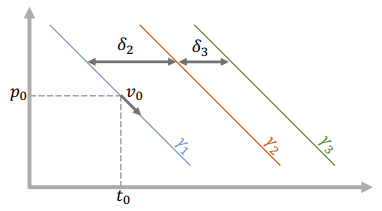
\includegraphics[width=3cm]{im1}} & \begin{tabular}{@{}l@{}} $g_p^k(u, v) = uv$ \\
					$\gamma_k(t) = p_0 + (t - t_0 - \delta_k)v_0$ \\
					$\eta_{k}^{\textbf{w}_{i}}(\psi_{i}(t_{ij})) = w_{ik} + p_{0} + (\alpha_{i}(t_{ij}-t_{0}-\tau_{i})+\delta_{k})v_{0}$ \end{tabular}\\
				\hline
				\multicolumn{2}{ |l| }{(b) Lineas rectas} \\
				\hline
				\raisebox{-0.6\height}{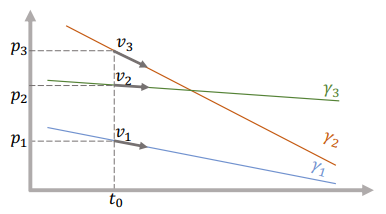
\includegraphics[width=3cm]{im2}} & \begin{tabular}{@{}l@{}} $g_p^k(u, v) = uv$ \\
					$\gamma_k(t) = p_k + (t - t_0)v_k$ \\
					$\eta_{k}^{\textbf{w}_{i}}(\psi_{i}(t_{ij})) = w_{ik} + p_{k} + \alpha_i(t_{ij}-t_{0}-\tau_{i})v_{k}$\end{tabular} \\
				\hline
				\multicolumn{2}{ |l| }{(c) Formas logísticas paralelas} \\
				\hline
				\raisebox{-0.6\height}{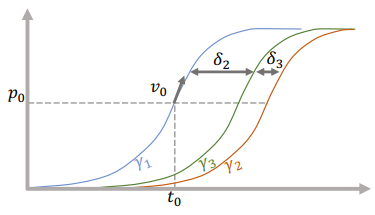
\includegraphics[width=3cm]{im3}} & \begin{tabular}{@{}l@{}} $g_p^k(u, v) = \frac{uv}{p^{2}(1-p)^{2}}$ \\
					$\gamma_k(t) = (1+(\frac{1}{p_{0}}-1)E(t))^{-1}$ \\
					$\eta_{k}^wi(\psi_i(t_{ij})) = (1+(\frac{1}{p_{0}}-1)\exp (\frac{-v_{0}(\alpha_{i}(t-\tau_{i}-t_{0})+\delta_{k})}{p_{0}(1-p_{0})}-\frac{w_{ik}(1+gE(t_{0}))^{2}}{gE(t_{0})}))^{-1}$\end{tabular} \\
				\hline
				\multicolumn{2}{ |l| }{(d) Formas logísticas} \\
				\hline
				\raisebox{-0.6\height}{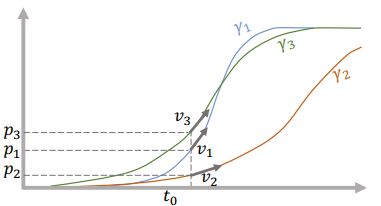
\includegraphics[width=3cm]{im4}} & \begin{tabular}{@{}l@{}} 
					$g_p^k(u, v) = \frac{uv}{p^{2}(1-p)^{2}}$\\
					$\gamma_k(t) = (1+(\frac{1}{p_{k}}-1)\exp(-\frac{v_{k}}{p_{k}(1-p_{k})}(t-t_{0})))^{-1}$ \\
					$\eta_{k}^wi(\psi_i(t_{ij})) = (1+(\frac{1}{p_{k}}-1)\exp (-\frac{w_{ik}+v_{k}\alpha_{i}(t_{ij}-\tau_{i}-t_{0})}{p_{k}(1-p_{k})}))^{-1}$\end{tabular} \\
				\hline
				\multicolumn{2}{ |l| }{(e) Decaimientos exponenciales paralelos} \\
				\hline
				\raisebox{-0.6\height}{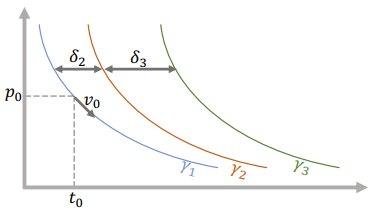
\includegraphics[width=3cm]{im5}} & \begin{tabular}{@{}l@{}} 
					$g_p^k(u, v) = \frac{uv}{p^{2}}$ \\
					$\gamma_k(t) = p_{0}\exp(-\frac{v_{0}}{p_{0}}(t-t_{0}+\delta_{k}))$ \\
					$\eta_{k}^wi(\psi_i(t_{ij})) = p_{0}\exp(-\frac{w_{i}k}{p_{0}}-\frac{v_{0}}{p_{0}}(\alpha_{i}(t_{ij}-t_{0}-\tau_{i})+\delta_{k}))$\end{tabular} \\
				\hline
				\multicolumn{2}{ |l| }{(f) Decaimientos exponenciales} \\
				\hline
				\raisebox{-0.6\height}{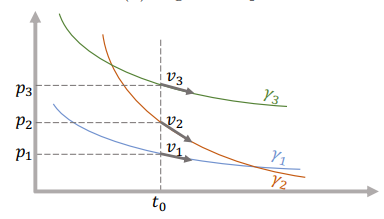
\includegraphics[width=3cm]{im6}} & \begin{tabular}{@{}l@{}} 
					$g_p^k(u, v) = \frac{uv}{p^{2}}$ \\
					$\gamma_k(t) = p_{k}\exp(-\frac{v_{k}}{p_{k}}(t-t_{0}))$ \\
					$\eta_{k}^wi(\psi_i(t_{ij})) = p_{k}\exp(-\frac{w_{ik}}{p_{k}}-\frac{v_{k}\alpha_{i}}{p_{k}}(t_{ij}-t_{0}-\tau_{i}))$\end{tabular} \\
				\bottomrule
			\end{tabular}
		\end{adjustbox}
		\caption{Instanciaciones del modelo genérico}
		\label{tab:tabla1}
	\end{table}
	
	
	\subsection{Modelo de Progresión de la Enfermedad (DPM)}
	En la tabla \ref{tab:tabla1} vemos seis distintas formas de instanciar el modelo genérico: 
	\begin{enumerate}
		\item \textbf{Lineas rectas paralelas.} Cada geodésica \textit{k} realiza una traslación horizontal de valor $\delta_{k}$ y alcanzan el valor $p_{0}$ con velocidad $v_{0}$ y tiempo $t_{0}+\delta_{k}$.
		\item\textbf{ Lineas rectas.} Representan geodésicas que alcanzan el valor $p_{k}$ con velocidad $v_{k}$ en el tiempo $t_{0}$.
		\item \textbf{Formas logísticas paralelas.} \textit{K} dimensiones representadas por curvas logísticas con valores entre 0 y 1, retrasadas por un tiempo $\delta_{k}$ y que alcanzan $p_{0}$ en el tiempo $t_{0}$ con velocidad $v_{0}$.
		\item \textbf{Formas logísticas.} Cada coordenada es independiente, alcanzando el valor $p_{k}$ en el tiempo $t_{0}$ con velocidad $v_{k}$.
		\item \textbf{Decaimientos exponenciales paralelos.} Geodésicas como curvas exponenciales decrecientes que van desde $-\infty$ finalizando en 0, trasladadas las curvas \textit{k} un tiempo $\delta_{k}$.Alcanzan $p_{0}$ con $v_{0}$ en t igual a $t_{0}$.
		\item \textbf{Decaimientos exponenciales.} Alcanzan el valor $p_{k}$ en el tiempo $t_{0}$ con velocidad $v_{k}$.
	\end{enumerate}
	
	En cada uno de ellos se refleja la función de $g_{p}^{k}$, la ecuación de la geodésica de una dimensión $\gamma_{k}$  y la coordenada k de la trayectoria individual $\eta_{k}^{\textbf{w}_{i}}(\psi_{i}(t_{ij}))$. \\
	
	Para cambiar estos seis modelos se pueden realizar algunas variaciones disponibles en softwares como Leaspy. Entre ellas encontramos las siguientes:
	\begin{itemize}
		\item Parametrización de formas distintas aplicables a los distintos modelos: valor $p_{0}$ alcanzado con velocidad $v_{0}$ en distintos momento, o valores $p_{1}$ a $p_{n}$ alcanzados por un solo momento.
		\item Modelos univariantes en los que establecer $\textbf{w}_{i}=(\textbf{w}_{i1})=0$ para poder usar los modelos mencionados.
		\item Número de fuentes ($\textit{N}_{S}$) las cuales definen el subespacio de posibles direcciones para el desplazamiento espacial. El valor ideal de esta variable es el mínimo que consigue saturar el ruido.
	\end{itemize}
	
	Una vez conocemos las distintas opciones de modelos posibles, es necesario saber como reconocer cual es el que mejor cumple las necesidades. Entre los factores a considerar están el proceso biológico en cuestión, el número de sujetos del estudio y el numero de puntos temporales disponibles en los datos. Tener en cuenta todo esto es necesario para escoger un modelo que represente con precisión la población estudiada y su evolución.\\
	
	
	
	
	
	\section{Estimation}
	\subsection{Aprendizaje estadístico y algoritmos}
	En primer lugar, el siguiente modelo correspondiente al i-ésimo sujeto, representa la dependencia de su variable de salida ($y_{i}$) en función de las variables aleatorias del mismo ($z_{i}$) y de los parámetros del modelo($\theta$). Para datos longitudinales, el grupo de observaciones en distintos momentos es $y_{i}=(y_{ij})_{j}$
	\begin{equation}
		y_{i}=f(\theta,z_{i})+\epsilon_{i}
	\end{equation}
	
	El principal objetivo es maximizar la verosimilitud buscando los parámetros que mejor describan las observaciones. Para ello, se desarrollaron diferentes algoritmos que se encargan de estimar los parámetros de modelos estadísticos. Cada uno centrado en resolver desafíos específicos utilizando enfoques iterativos:
	
	\begin{description}
		\item {\textbf{Algoritmo E-M: }}Expectation-Maximization.\\
		Debido a la dependencia con variables latentes \textit{z}, que suelen ser desconocidas, es complicado maximizar la verosimilitud directamente. Para solucionar esto, con este algoritmo se itera alternando entre el paso de Expectación, encargado de calcular a partir de $\theta(0))$  la expectativa de las variables latentes, y el paso de Maximización, que haya los parámetros $\theta(k)$ para maximizar la función anterior.
		
		\item {\textbf{Algoritmo SAEM: }}Stochastic Approximation Expectation Maximization.\\
		Desarrollado debido a la difícil optimización de la verosimilitud en modelos no lineales con variables latentes. Consiste en sustituir el paso de Expectación del algoritmo anterior por el de Aproximación Estocástica. En este se utilizan muestras $z^{k}$ para acercarse a la cantidad deseada. Además, tiene una fase de "quemado" al inicio, que opera con:
		\begin{equation}
			\mathcal{Q}_{k}(\theta)=log\ p(y,z^{(k)};\theta)
		\end{equation}
		
		crucial para explorar el espacio de soluciones. También realiza la actualización iterativa de los parámetros.
		
		\item {\textbf{Algoritmo MCMC-SAEM: }}Monte Carlo Markov Chain SAEM.\\
		Surge debido la posibilidad de que $p(z|y;\theta^{(k)})$ sea desconocida. Mediante el teorema de Bayes, se expresa en función de términos del modelo, del valor previo de variables ocultas y una constante de normalización.
		\begin{equation}
			p(\mathbf{z}|\mathbf{y};\theta^{(k)})=\frac{p(\mathbf{y}|\mathbf{z};\theta^{(k)})p(\mathbf{z};\theta^{(k)})}{p(\mathbf{y};\theta^{(k)})}
		\end{equation}
		Para solucionar esto, primero se realiza la aproximación de las muestras $z^{(k+1)}$  que sigan la distribución $p(z^{(k)}|y;\theta^{(k)})$, con el algoritmo de Metropolis-Hasting mediante el método de cadena de Markov. También se sustituye el procedimiento de muestreo por el MCMC y se hace converger hacia un punto crítico de verosimilitud observada $p(y|z)$ con el algoritmo de MCMC-SAEM. Para simplificar el logaritmo de verosimilitud se establece que el modelo pertenece a la familia exponencial. Además, solo se calcula y propaga el vector $\mathit{S}(\mathbf{y},\mathbf{z})$ para lograr una reducción computacional y se actualizan los parámetros $\theta^{(k+1)}$ en la Maximización. \cite[Capítulo 2]{koval2020learning}
		
		\item {\textbf{Algoritmo Hasting Metropolis within Gibbs sampler }}\\
		En el caso de variables multivariadas se puede complicar el muestreo de $z^{(k)}$ mediante cadena de Markov. Por ello, se desarrolló este algoritmo en el que $\mathbf{z}=(\mathbf{z}_{l})_{1\leq l\leq L}$ y $p(\mathbf{z}_{l}|\mathbf{z}_{\bar{l}}, \mathbf{y};\theta)$ es conocida hasta una constante $(\mathbf{z}_{\bar{l}}=\mathbf{z} \backslash \{{\mathbf{z}_{l}}\})$, pudiendo muestrear las coordenadas de $\mathbf{z}$. Al realizar el muestreo utilizando el muestreador de Hastings-Metropolis se llega al algoritmo de Hastings-Metropolis dentro del muestreador de Gibbs.
	\end{description}
	
	\subsection{Estimación del modelo de progresión de la enfermedad}
	En la siguiente ecuación, se ve un modelo de efectos mixtos de progresión espacio-temporal parametrizado por $\theta_{geom}$ (parámetros geométricos) y $z_{i}$ (variables ocultas individuales de la variación en la progresión promedio grupal). Estas últimas dan lugar a un conjunto global de parámetros $\theta=(\theta_{geom}, \theta_{\mathbf{z}})$.
	\begin{equation}
		y_{ij}=f(\theta_{geom},\mathbf{z}_{i},t_{ij})+\epsilon_{ij}
	\end{equation}
	
	donde:
	\begin{equation}
		\epsilon_{ij} \sim \mathcal{N}(0, \gamma^{2})
	\end{equation}
	
	La verosimilitud del modelo se formula de la siguiente forma:
	\begin{equation}
		p(\mathbf{y};\theta) = \int p(\mathbf{y}|\mathbf{z};\theta)p(\mathbf{z};\theta)dz
	\end{equation}
	
	A raíz de esto, se caracterizan los siguientes procesos estadísticos:
	\begin{description}
		\item {\textbf{Calibración.}}\\
		En esta fase, el objetivo es calcular los parámetros $\hat{\theta}$ para maximizar la verosimilitud del modelo de progresión de la enfermedad y su variabilidad. Para converger hacia un máximo local en la distribución posterior, se usa el algoritmo MCMC-SAEM (variables ocultas desconocidas y supuesto modelo de familia exponencial). \\
		
		Para este proceso, es importante tener en cuenta lo siguiente:
		\begin{itemize}
			\item Identificabilidad estructural: asegura que no haya varios grupos de parámetros generando la misma distribución.
			\item Identificabilidad práctica: Está relacionado con la calidad y la cantidad de las medidas. Para afrontar problemas en esta parte de nuestro modelo, se realiza una reparametrización.
		\end{itemize}
		\item {\textbf{Personalización.}}\\
		Consiste en maximizar la verosimilitud:
		\begin{equation}
			p(\mathbf{y}_{i}, \mathbf{z}_{i};\hat{\theta})=p(\mathbf{y}_{i}| \mathbf{z}_{i};\hat{\theta})p( \mathbf{z}_{i};\hat{\theta})
		\end{equation} 
		
		calculando el mejor valor de los efectos aleatorios $\mathbf{z}_{i}^{*}$, teniendo en cuenta un conjunto de datos longitudinales \textit{\textbf{y}} y $\hat{\theta}$ que maximiza $p(\mathbf{y},\theta)$. Dos procedimientos utilizados para la optimización son el método L-BFGS o el método de Powell. Otra alternativa es iterar \textit{K} veces con los parámetros individuales el algoritmo MCMC-SAEM.\\
		
		Que el individuo personalizado pertenezca o no al conjunto de calibración deriva en la práctica en resultados similares. Por otra parte, a mayor numero de observaciones del sujeto, mayor es la posibilidad de las mediciones individuales difieran del promedio del grupo.	
		
		\item {\textbf{Reconstrucción, imputación de valores faltantes y predicción.}}\\
		Una vez obtenida la trayectoria espacio-temporal individual, a partir de $\mathbf{z}_{i}^{*}$ devuelto por el proceso de personalización, se realiza uno de los siguientes procesos dependiendo del rango de tiempos con el que se trabaje:
		\begin{itemize}
			\item Reconstrucción ($t_{i1}<t<t_{ik_{i}}$): Reconstruye los dato del modelo $y_{ij}^{*}=f(\theta, \mathbf{z}_{i}^{*}, t_{ij})$, apareciendo un error $||y_{ij}-y_{ij}^{*}||$.
			\item Imputación de valores faltantes ($t_{i1}<t<t_{ik_{i}}$ y $t \notin \{t_{i1},...,t_{ik_{i}}\}$): Calcula valores que no se han encontrado en el conjunto inicial $y_{ij}^{*}=f(\theta, \mathbf{z}_{i}^{*}, t_{ij})$.
			\item Predicción ($t>t_{ik_{i}}$): Calcula las medidas en tiempos futuros, cuya precisión se basa en querer traspasar el escenario a largo plazo grupal a cada individuo. Es poco realista predecir etapas que estén fuera de la base de datos de entrenamiento, por ser dinámicas desconocidas.
		\end{itemize}
		
		\item {\textbf{Simulación.}}\\
		Por último, tras haber obtenido los parámetros óptimos $\hat{\theta}$ y las variables ocultas individuales, se realiza este procedimiento para simular sujetos virtuales. Esto permite crear cohortes con mayor numero de pacientes, de visitas y una mayor precisión temporal. Para saber la calidad de la cohorte simulada la comparamos con la distribución de las variables ocultas y las salidas finales de la cohorte original. Esta funcionalidad también permite corregir sesgos, como por ejemplo el incluir preferentemente pacientes con más visitas. 
	\end{description}
	
	
	
	\section{Estimation of the Disease Progression Model}
	
	Para el análisis de datos con estructura espacial con el objetivo de estimar el
	avance de enfermedades, así como para el estudio de datos longitudinales se
	desarrollaron las siguientes herramientas de software: Leasp para C++ y Leaspy
	para Python. El segundo es utilizado mayoritariamente para estimar la progresión
	de enfermedades a largo plazo, imputar valores faltantes y la simulación de
	cohortes virtuales.\cite[Capítulo 7]{koval2020learning}
	
	\subsection{Leasp: Paquete de C++ para el Análisis de Datos Longitudinales Estructurados Espacialmente}
	
	Este paquete trabaja con datos obtenidos tras la observación de pacientes a lo
	largo del tiempo. Su función se basa en: reconstruir la trayectoria a largo
	plazo de los pacientes a partir de las observaciones, ubicar cada medida de cada
	paciente en relación con la linea de tiempo promedio grupal y medir el efecto de
	ciertos cofactores como por ejemplo el género en el transcurso de la señal.\\
	
	Esta herramienta puede trabajar tanto con variables escalares, como puntuaciones
	clínicas o evaluaciones cognitivas; como con 	datos de red (PET SUVR).\\
	
	El diseño de Leasp se centra en la interacción entre un algoritmo y un modelo
	basado en entradas escalares y de red. Con esta biblioteca se tiene acceso a
	distintas carpetas que permite el uso de varias funcionalidades:
	\begin{itemize}
		\item Aplicación de procedimientos matemáticos
		\begin{itemize}
			\item Calibración
			\item Personalización
			\item Simulación
		\end{itemize}
		\item Funciones de procesamiento
		\item Herramientas de visualización
	\end{itemize}
	
	Para su correcta utilización a continuación se muestran algunas instrucciones y
	pasos que se deben seguir:
	
	\begin{description}
		\item {\textbf{Requisitos.}} Es necesario instalar las siguientes bibliotecas:
		\textit{tinyxml} (lectura y preprocesamiento de archivos xml),
		\textit{googletest} (pruebas de unidad y funcional ) y  \textit{Armadillo} (uso
		de algebra lineal para vectores y matrices) 
		
		\item {\textbf{Instalación.}} Desde la terminal, ejecutar los comandos que se
		muestran a continuación:
		\begin{enumerate}
			\item \texttt{git clone https://gitlab.com/icm-institute/aramislab/leasp}
			\item \texttt{git submodule init}
			\item \texttt{git submodule update}
			\item \texttt{. mkdir build \&\& cd build}
			\item \texttt{. cmake --options}
			\item \texttt{. make --options\}}
		\end{enumerate}
		
		\item {\textbf{Ejecución del software.}} Agregación del software a
		\texttt{/protect/T1/textdollarPATH} y ejecucion del siguiente comando:
		\begin{center}
			\texttt{leasp fit model\_stgs.xml algorithm\_stgs.xml data\_stgs.xml sampler\_stgs.xml}
		\end{center}
		
		\begin{itemize}
			\item \texttt{fit}: Ajuste de la curva promedia grupal a medidas individuales.
			\item \texttt{model\_settings}: Da información de los parámetros y del tipo de modelo	que se va a ejecutar.
			\item \texttt{algorithm\_settings.xml}: Define parámetros del algoritmo como el numero total de iteraciones.
			\item \texttt{data\_settings.xml}: Recopila la ruta de los archivos de datos.
			\item \texttt{sampler\_settings.xml}: Enumera las muestras utilizadas en el procedimiento de estimación, junto con sus parámetros.
		\end{itemize}
		
		\item {\textbf{Salidas de la estimación.}} Se producen tres archivos en el proceso: \\
		\texttt{convergence\_parameters.csv} muestra la convergencia del modelo.\\ \texttt{population\_parameters.csv} define parametros para el promedio grupal a largo plazo.\\ \texttt{individual\_parameters.csv} que son parametros temporales y espaciales para la trayectoria individual.
	\end{description}
	
	\subsection{Leaspy: Toolbox de Python para Aprender Patrones Espaciotemporales de la Progresión de la Enfermedad}
	
	Para el estudio de datos longitudinales y ver la progresión de enfermedades a largo plazo en Python se desarrollo la herramienta Leaspy. Basándose en el modelo de efectos mixtos, permite la reconstrucción de la evolución promedia e individual. Además, permite abordar problemas de los estudios de datos longitudinales, como el que cada paciente tenga un numero de observaciones distinto, permite trabajar con valores faltantes y medidas de datos estructurados espacialmente (imágenes o redes), gracias a la geometría de Riemann. También es de gran utilidad trabajando con medidas en un periodo de tiempo corto, cuando el fenómeno de estudio es de larga duración. Otras aplicaciones permiten predecir puntos temporales futuros y simular nuevas cohortes a partir de los parámetros obtenidos de un ya existente. La calidad del paquete se garantiza mediante pruebas unitarias, control de versiones git e integración continua.\\
	
	El siguiente modelo, basado en efectos mixtos, representa un conjunto de datos longitudinales $y=(y_{ij},t_{ij})\ 1 \leq i \le n, 1 \le j \le k_{i}$ de $\textit{n}$ pacientes. El número de observaciones de cada individuo $i$ se representa con $k_{i}$, siendo los tiempos de cada observación $t_{i1} < ... < t_{ik_{i}}$.
	
	\begin{equation}
		y_{ij} = f(\theta_{geom}, z_{i}, t_{ij} ) + \epsilon_{ij}
	\end{equation}
	
	$\theta_{geom}$ son los parámetros del modelo, $z_{i}$ es la variación de cada individuo respecto a la trayectoria promedio grupal y $\epsilon_{ij}$ es un ruido gaussiano. El objetivo es calcular los parámetros anteriores que hagan que los datos sean lo más verosímiles posibles. Con Leaspy se pueden realizar los siguientes procedimientos:
	\begin{enumerate}
		\item Calibración: consiste en estimar $y$ a partir de $\theta$, obteniendo la curva promedio del grupo a largo plazo. Esta basada en el algoritmo MCMC-SAEM y la varianza adaptativa y el descenso de gradiente mejoran la velocidad de convergencia.
		\item Personalización: Teniendo $\hat{\theta}$, se reconstruyen las trayectorias individuales obteniendo la variable oculta $z_{i}^{*}$. Este procedimiento estadístico incluye métodos Powell y L-BFGS.
		\item Reconstrucción, imputación de valores faltantes y predicción: Con las variables resultantes de los dos pasos anteriores, se calcula $y_{ij}^{*}=f(\hat{\theta}, z_{i}^{*}, t_{ij})$ para distintos periodos de tiempo.
		\item Simulación: Se genera un individuo completamente nuevo ($z_{i}^{0}$) a partir de $\hat{\theta}$ y un conjunto de variables individuales, pudiendo repetir el proceso hasta conseguir una cohorte virtual. Este método está basado en estimaciones condicionales gaussianas multivariadas y en funciones de densidad kernel.	
	\end{enumerate}
	
	La programación en Python de los cuatro procesos anteriores sigue una metodología bastante amigable para le usuario, ya que menos para la reconstrucción, el resto se estructuran de la siguiente manera:
	\begin{itemize}
		\item \textbf{Definición de parámetros:} el objeto \texttt{AlgorithmSettings} se encarga de esta función. En su llamada se fija el algoritmo que se quiere utilizar y otras variables. También se pueden cargar a través de kwargs o archivos json.
		\item \textbf{Llamada a las funciones:} tras el paso anterior, se realiza la llamada al método que se este llevando a cabo, introduciendo los parámetros definidos: \texttt{leaspy.fit(...)} para la calibración, \texttt{leaspy.personalize(...)} para personalizar el modelo, \texttt{leaspy.reconstruct(...)} para reconstruirlo y\\\texttt{leaspy.simulate(...)} para realizar una simulación.
		\item \textbf{Visualización y registro:} Leaspy también permite guardar archivos de registro y otras variables en archivos csv y json, lo que también permite volver a cargarlos en el programa; y se pueden visualizar perfiles de progresión o reconstrucciones de trayectorias.
	\end{itemize}
	
	Con todas estas herramientas, Leaspy es un entorno versátil y de fácil acceso que permite introducirse en el mundo del análisis y la interpretación de datos longitudinales a través de Python. Permite abordar tareas estadísticas gracias a los modelos y algoritmos en los que esta basado , pudiendo estimara parámetros y simular datos. Además es accesibles desde distintos sistemas operativos como Windows o Linux.
	
\section{Robust parametric modeling of Alzheimer's disease progression (Alzheimer's RPDPM)}

La enfermedad de Alzheimer (EA) es una demencia progresiva que comienza en el hipocampo, con biomarcadores en el líquido cefalorraquídeo (LCR) que pueden volverse anormales antes de que los cambios sean detectables en la tomografía por emisión de positrones (PET) o la resonancia magnética (MRI). El modelo de progresión de la enfermedad (DPM) se basa en estudios longitudinales para describir cómo evoluciona la EA, utilizando métodos paramétricos que suponen una evolución sigmoidea de los biomarcadores y enfoques más flexibles como los procesos gaussianos. Este estudio mejora el modelo propuesto por Jedynak al introducir una extensión robusta utilizando la estimación M y una función logística modificada, superando los métodos anteriores y ofreciendo un enfoque más eficaz para la investigación y el diagnóstico clínico de la EA \cite{ghazi2021robust}.\\

\subsection{Método}

El estudio propone un modelo robusto de progresión de la enfermedad basado en una función logística ajustada por estimación M para manejar valores atípicos. Este modelo estima los valores de los biomarcadores \( y_{i,j,k} \) en función de un "Disease Progression Score" (DPS) calculado a partir de la edad del sujeto. La relación entre el biomarcador y el DPS se modela como:

\begin{equation}
	y_{i,j,k} = f(s_{i,j}; \theta_k) + \sigma_k \epsilon_{i,j,k},
\end{equation}


donde \( f(s_{i,j}; \theta_k) \) es una función logística que describe la dinámica del biomarcador, y

\begin{equation} 
	s_{i,j} = \alpha_i t_{i,j} + \beta_i,
\end{equation}


es el DPS, donde \( t_{i,j} \) representa la edad, \( \alpha_i \) la tasa de progresión y \( \beta_i \) el inicio de la progresión.\\

La optimización del modelo se realiza minimizando una función objetivo que combina el ajuste de los parámetros del biomarcador y del sujeto utilizando una función de máxima verosimilitud. El proceso de optimización alterna entre el ajuste de los parámetros del biomarcador y los parámetros específicos del sujeto hasta que se alcanza la convergencia.\\

Para la predicción del valor del biomarcador y la clasificación clínica, el modelo utiliza los parámetros ajustados y una función logística para predecir los biomarcadores. La clasificación del estado clínico se realiza utilizando un clasificador bayesiano con estimación de densidad (KDE) \cite{parzen1962estimation}, calculando la probabilidad posterior con:

\begin{equation}
	p(c_i \mid s) = \frac{p(c_i) p(s \mid c_i)}{\sum_i p(c_i) p(s \mid c_i)}
\end{equation}

donde \( p(c_i) \) es la probabilidad previa y \( p(s \mid c_i) \) es la probabilidad ajustada. Este enfoque proporciona un sistema sólido y eficaz para modelar y clasificar enfermedades \cite{ghazi2021robust}.

\subsection{Configuración experimental}
\subsubsection{Datos}

El estudio utiliza datos de dos iniciativas importantes: ADNI y NACC. ADNI, lanzada en 2003, combina MRI, PET, biomarcadores y evaluaciones clínicas para estudiar la progresión del deterioro cognitivo y el Alzheimer, clasificando a los sujetos en cognitivamente normales (CN), deterioro cognitivo leve (DCL) y enfermedad de Alzheimer (EA). NACC, desde 1999, recopila datos similares y los clasifica en las mismas categorías en función del estado de la enfermedad.\\

Los datos se filtraron para eliminar valores atípicos y grandes brechas de tiempo, lo que dio como resultado 1.518 sujetos ADNI y 239 NACC con al menos una prueba cognitiva. Las mediciones de MRI volumétricas se ajustaron para corregir las diferencias en el tamaño de la cabeza mediante análisis de covarianza. Los datos se dividieron en conjuntos de entrenamiento y prueba, y se aplicó el método \textit{bootstrap} para estimar la varianza.

\subsubsection{Ajuste}
En cuanto al algoritmo, los parámetros se inicializan como \(\alpha^{(0)} = 1\) y \(\beta^{(0)} = 0\). La pendiente de las trayectorias \(\lambda\) se establece en -1 o 1, según los diagnósticos. Los parámetros de las funciones logísticas se estiman como \(\gamma_k = 1\), \(c_k = 0\) y \(b_k = \frac{a_k - d_k}{4 \lambda_k}\), y el procedimiento alterno se repite durante un máximo de 30 iteraciones.\\

Para evitar el sobreajuste, se seleccionan los valores óptimos de los parámetros en función de la pérdida de validación óptima \cite{prechelt2002early}:

\begin{equation}
	\{\alpha^*, \beta^*, \theta^*\} = \arg\min_{L_{\text{min}} \leq l \leq L_{\text{max}}} E_{\text{valid}}(l)
\end{equation}

donde \(E_{\text{valid}}(l)\) es la pérdida de validación en la \(l\)ª iteración. El número mínimo de iteraciones es 10 y el máximo es 50.

\subsubsection{Evaluación}
Entre las distintas métricas utilizadas para medir la precisión de las estimaciones realizadas mediante RPDPM ('Robust Parametric Disease Progression Modeling') se encuentran: 
\begin{enumerate}
	\item Criterio de información Bayesiano Robusto (BIC): utilizado parala selección de modelos entre los modelos robustos. \cite{9225726}
	\item Error Absoluto Medio (MAE): Mide la precisión de la trayectorio de la enfermedad estimada para los biomarcadores.
	\item Área  bajo la curva (AUC) de la característica operativa del receptor (ROC): mide el rendimiento diagnóstico.
\end{enumerate}

\begin{table}[h!]
	\centering
	\begin{tabular}{|c|c|}
		\hline
		\textbf{Nombre} & \textbf{Ecuación} \\
		\hline
		\text{BIC} & \( \text{BIC} = 2 E_{\text{train}}(L_{\text{opt}}) + Q \ln(N) \) \\
		\hline
		\text{MAE} & \( \text{MAE} = \frac{1}{N_k} \sum_{(i,j) \in N_k} \left| y_{i,j,k} - f(s_{i,j}; \theta_k) \right| \) \\
		\hline
		\text{AUC} & \( \text{AUC} = \frac{1}{n_c (n_c - 1)} \sum_{i=1}^{n_c - 1} \sum_{k=i+1}^{n_c} \frac{1}{n_i n_k} \left( SR_i - \frac{n_i (n_i + 1)}{2} + SR_k - \frac{n_k (n_k + 1)}{2} \right) \) \\
		\hline
	\end{tabular}
	\caption{Métricas de evaluación del RPDPM.}
\end{table}

siendo \(E_{\text{train}}(L_{\text{opt}})\) la pérdida de entrenamiento, \(N\) el número total de mediciones, \(Q\) el número total de parámetros, \(N_k\) es el número de mediciones para el biomarcador \(k\), \(y_{i,j,k}\) es el valor real, y \(f(s_{i,j}; \theta_k)\) es el valor estimado, \(n_c\) el número de clases, \(n_i\) el número de observaciones en la \(i\)-ésima clase y \(SR_i\) es la suma de los rangos de las probabilidades posteriores.\\

\subsection{Resultados y discusión}
El modelo propuesto se aplicó para analizar la dinámica de los biomarcadores de la enfermedad de Alzheimer utilizando datos de ADNI. Este modelo, basado en una función Stannard modificada y una función de pérdida logística, mostró un rendimiento superior en términos de BIC y NMAE, lo que justifica su uso en análisis posteriores.\\

El análisis temporal de los biomarcadores reveló que los biomarcadores de CSF, PET y RAVLT-IR aparecen antes que los de MRI y pruebas cognitivas. Los puntos de inflexión en las curvas de biomarcadores ayudaron a ordenar su aparición a lo largo de la enfermedad, aunque no detectaron anomalías tempranas.\\

El modelo también se destacó en la predicción de valores de biomarcadores y la clasificación del estado clínico, logrando un AUC de 0,931, mejorando así en precisión y robustez. En comparación con otros métodos, superó a los enfoques anteriores en AUC y MAE para ADAS-13, aunque tuvo un rendimiento menor en la predicción de volúmenes ventriculares normalizados.\\

Finalmente, el modelo mostró una buena capacidad de generalización cuando se aplicó a datos NACC, demostrando un desempeño superior a los modelos anteriores, lo que sugiere su robustez y adaptabilidad a diferentes cohortes.

\subsection{Conclusión}
El artículo presenta un modelo paramétrico robusto para modelar la progresión del Alzheimer utilizando estimación alternada con pérdida logística para manejar problemas de ajuste como valores atípicos. Este método transforma las edades en puntuaciones de progresión de la enfermedad y ajusta funciones modificadas a biomarcadores longitudinales. Los resultados demostraron que el método propuesto supera las técnicas actuales en rendimiento predictivo y se generaliza bien a diferentes cohortes. El enfoque se puede adaptar a datos de series temporales con datos faltantes y se puede utilizar con biomarcadores no monótonos. También se sugiere que en lugar de estimadores M, se pueden utilizar estimadores robustos \cite{rousseeuw2005robust}, aunque esto requiere optimizar un parámetro adicional para el recorte residual.

\section{Aportación al desarrollo del TFG}
\subsection{Neurodegeneración: Alzheimer, Parkinson y ELA}
Esta sección aporta una definición de los que son las enfermedades neurodegenerativas, explicando algunas de ellas como el Alzheimer o el Parkinson. Esto sirve para sentar un contexto dentro del estudio intentando simplificar el funcionamiento del cerebro humano.\\

También trata la importancia de la anticipación a estas enfermedades para intentar prevenir el declive cognitivo, siendo esta una de las razones principales de este proyecto. La importancia de encontrar modelos predictivos que ayuden a estimar con antelación la evolución de la enfermedad de Parkinson y la aparición del declive cognitivo. \\

\subsection{Clinical variables and biomarkers in prediction of cognitive impairment in patients with newly diagnosed Parkinson’s disease: a cohort study}
Este artículo destaca la importancia de predecir el declive cognitivo en etapas tempranas, a partir de combinaciones de biomarcadores como MoCA, APOE, UPSIT, etc.\\

Además se utiliza como base de datos la PPMI (Parkinson's Progression Markers Initiative) también utilizada para este proyecto, lo que sirve como base para conocer los marcadores o combinaciones de biomarcadores que han tenido más poder para pronosticar la enfermedad y compararlos con los resultados obtenidos en este caso. También sirve como referencia sobre el estado actual de la investigación sobre la aparición del declive cognitivo en etapas tempranas del Parkinson.

\subsection{Statistical analysis of longitudinal neuroimage data with Linear Mixed Effects models}
Este documento aporta información sobre la utilización de modelos de efectos mixtos lineales (LME) en el análisis de datos longitudinales. Esto es crucial para analizar los cambios de los marcadores entre los distintos pacientes y durante las visitas que realizan los mismos en tiempos diversos, y así poder predecir la progresión del declive cognitivo.\\

Por otro lado, compara la precisión de este método con otros como el ANOVA de medidas repetidas, resaltando la potencia estadística al utilizar el LME, lo cual se puede usar de referencia a la hora de escoger la forma para analizar los datos utilizados en el trabajo. 

\subsection{Estimating long-term multivariate progression from short-term data}
En este artículo se trata la complejidad de estimar la progresión de una enfermedad neurodegenerativa a largo plazo a partir de datos a corto plazo, concretamente centrándose en el Alzheimer. Aún así, sirve como referencia para la aplicación para la misma problemática aplicada al Parkinson, observando los distintos métodos descritos y los resultados obtenidos.\\

\subsection{Modelos escalares y extensiones}
Este texto aporta conceptos matemáticos y estadísticos fundamentales a la hora de predecir el declive cognitivo y modelar la progresión del Parkinson. Por ejemplo, aporta información sobre la geometría de Riemann, la cual define el espacio de características formado por geodésicas que sirve para analizar la evolución individual de la enfermedad.También explica el funcionamiento de los modelos de efectos mixtos, lineales y no lineales.\\

Todas estas herramientas son combinadas para el Modelado de Progresión de la Enfermedad (DPM), por lo que una explicación de los mismo aporta un conocimiento en profundidad de los métodos con los que se trabajará para así poder obtener unas predicciones más exactas.

\subsection{Estimation}
Este documento aporta información sobre distintos métodos avanzados de gestión de la incertidumbre y variabilidad de los datos, como el Expectation-Maximization (E-M) o el Monte Carlo Markov Chain SAEM (MCMC-SAEM).\\

También explica como aplicarlos a la calibración, personalización, reconstrucción e imputación de datos faltantes, procedimientos cruciales para adaptar los modelos a datos individuales y que será muy útil en este proyecto.

\subsection{Estimation of the Disease Progression Model}
Este apartado aporta información sobre las herramientas \textit{Leasp} y \textit{Leaspy}, las cuales serán fundamentales para el desarrollo de este trabajo. Permiten analizar datos longitudinales mediante la reconstrucción de trayectorias a largo plazo e imputar valores faltantes, muy útil para evaluar el avance de la enfermedad.\\

Además, el entorno de Leaspy, en el que se centrará el desarrollo del algoritmo de Python, permite reconstruir trayectorias individuales y simular nuevos sujetos, facilitando la predicción de futuros puntos temporales.

\subsection{Robust parametric modeling of Alzheimer's disease progression (Alzheimer's RPDPM)}
Con este texto se introduce la aplicación del método RPDPM para predecir la progresión de la enfermedad del Alzheimer. Utiliza una función logística ajustada mediante estimación robusta para manejar valores atípicos y realizar predicciones precisas. \\

Los resultados mostrados se usarán como referencia para comparar los obtenidos, utilizando \textit{Leaspy}, para la problemática de la predicción del declive cognitivo en el Parkinson.

